\documentclass[10.9pt]{article}

\usepackage[paper=letterpaper,centering,margin=1.0in]{geometry}
\usepackage{setspace}

\usepackage[american]{babel}
\usepackage{epsfig,subfigure}
\usepackage{color,cite}
\usepackage{amsthm,amsfonts,amsmath,amssymb,amstext,latexsym}
\usepackage{multirow}
\usepackage{soul}
%\usepackage{xxcolor}
\usepackage{xcolor}
%\usepackage{hyperref}
\usepackage{algorithm}
\usepackage{algpseudocode}

\usepackage{graphicx}
\usepackage{amstext}

%\usepackage[utf8]{inputenc}
%\usepackage{enumitem}

%\algnewcommand{\IIf}[1]{\State\algorithmicif\ #1\ \algorithmicthen}
%\algnewcommand{\EndIIf}{\unskip\ \algorithmicend\ \algorithmicif}
\newcommand{\algorithmicbreak}{\textbf{break}}

\newcommand*{\Cdot}[1][1.25]{%
  \mathpalette{\CdotAux{#1}}\cdot%
}
\newdimen\CdotAxis
\newcommand*{\CdotAux}[3]{%
  {%
    \settoheight\CdotAxis{$#2\vcenter{}$}%
    \sbox0{%
      \raisebox\CdotAxis{%
        \scalebox{#1}{%
          \raisebox{-\CdotAxis}{%
            $\mathsurround=0pt #2#3$%
          }%
        }%
      }%
    }%
    % Remove depth that arises from scaling.
    \dp0=0pt %
    % Decrease scaled height.
    \sbox2{$#2\bullet$}%
    \ifdim\ht2<\ht0 %
      \ht0=\ht2 %
    \fi
    % Use the same width as the original \cdot.
    \sbox2{$\mathsurround=0pt #2#3$}%
    \hbox to \wd2{\hss\usebox{0}\hss}%
  }%
}


%\algdef{SE}[SUBALG]{Indent}{EndIndent}{}{\algorithmicend\ }%
%\algtext*{Indent}
%\algtext*{EndIndent}



\newcommand{\squishlist}{
 \begin{list}{$\bullet$}
  { \setlength{\itemsep}{0pt}
     \setlength{\parsep}{3pt}
     \setlength{\topsep}{3pt}
     \setlength{\partopsep}{0pt}
     \setlength{\leftmargin}{1.5em}
     \setlength{\labelwidth}{1em}
     \setlength{\labelsep}{0.5em} } }

\newcommand{\squishend}{
  \end{list}  }

\newtheorem{theorem}{Theorem}
\newtheorem{lemma}{Lemma}
\newtheorem{conjecture}{Conjecture}
\newtheorem{remark}{Remark}
% \newtheorem{proof}{Proof}
\newtheorem{proposition}{Proposition}
\newtheorem{observation}{Observation}
\newtheorem{definition}{Definition}
\newtheorem{corollary}{Corollary}
\newtheorem{assumption}{Assumption}

\newcommand{\bydef}{\stackrel{\rm{def}}{=}}
%\newcommand{\textul}[1]{\underline{#1}}

\newcommand{\cP}{{\cal P}}
\newcommand{\cR}{{\cal R}}
\newcommand{\cK}{{\cal K}}
\newcommand{\norm}[1]{\left\Vert#1\right\Vert}
\newcommand{\mc}[1]{\mathcal{#1}}
\newcommand{\Lrz}{\mbox{${\mathbb L}$}}
\newcommand{\DMU}{\text{DMU}}


% Comments colors conventions
\newcommand{\J}[1]{{\textcolor{cyan}{#1}}}
\newcommand{\JC}[1]{\textbf{{\textcolor{red}{Juan: #1}}}} 
\newcommand{\SAB}[1]{\textbf{{\textcolor{orange}{Sab: #1}}}} 

\newcommand{\preg}[1]{\textbf{{\textcolor{blue}{Sab: #1}}}} 


\def\R{\mbox{${\mathbb R}$}}           % Real numbers
\def\N{\mbox{${\mathbb N}$}}           % Natural numbers
\def\Z{\mbox{${\mathbb Z}$}}           % Integer numbers

\def\E{\mbox{${\mathbb E}$}}           % Expected value


\title{ Whisper Project \\ 
\begin{large} - Final Report - }

\author{
\begin{center}
    \begin{tabular}[c]{  p{3.3cm}  p{3.3cm}  p{3.3cm} }
		Fernando Villa & Khalid Alobaid & Mariya Abdiyeva \\
		Nicolas Cabuli & Oluremi Obolo & Santiago Arrubla
    \end{tabular}
\end{center}
}



%\author{Fernando Villa \and Khalid Alobaid \and Mariya Abdiyeva \and Nicolas Cabuli \and Oluremi Obolo \and Santiago Arrubla}

\begin{document}
\date{30 March 2017}
\maketitle


\section{Introduction}
\label{sec:part 1}

\subsection{Requirements (Aims)}

Our aim is to create a distributed chat system with the following specific requirements by  priority.

\begin{table}[ht]
\caption{Requirements by priority level}
\label{tab:requirements}
    \begin{tabular}[c]{ | p{5cm} | p{5cm} | p{5cm} |}
		\hline
		\centering\textbf{Priority 1} & \centering{\textbf{Priority 2}} & \centering\textbf{Priority 3} &
    \hline
    \parbox[t]{5cm}{-Secure connection\\-Encrypted messages\\ -iOS, Android and Web platforms (at least two platforms)\\ -Contact list\\ -Search for contacts\\ -Sign in by email or Gmail \\ -One to one conversation (text message)} &  \parbox[t]{5cm}{-Send images\\ -Group chat\\ -Chat bubbles instead of username\\ -Notifications of received messages}
& \parbox[t]{5cm}{-Sign Up with Facebook\\ -Availability to send other type of media (e.g. video, voice notes, etc.)\\ -Online status of other users\\ -Acknowledgment of received, delivered and read messages, including date time\\ -Ability to use the chat offline}\\
    \hline
    \end{tabular}
\end{table}


\subsection{Strategy and Timetable}

Our strategy is to develop three client-based platforms (i.e. Android, iOS and Web) using Firebase as a server. The reason for including a third platform is to act as a backup should there be problem with any of the platforms during testing which we are unable to debug at the end. The tentative timetable (Figure ~\ref{fig:timetable}) presents the main activities required to complete our final product. It is important to state that the timetable and our strategy is constructed based on the Scrum ~\cite{scrum} methodology, which  is an agile software development guide that allows us to iterate and make incremental and evolutionary contributions.  We will also use different Project Management roles like a Scrum Master (who removes team obstacles and pushes resolutions) and the product owner (who acts as the client voice) to ensure a high-quality product. The main activities are explained as follows: 

\begin{enumerate}
	\item \textbf{Plan}: Here we defined how we are going to work, our goals and organization as a team. We also discussed our individual strengths and weaknesses and the tools available to achieve our aim and objectives.
	\item \textbf{Firebase}: For simplicity, costs (free) and security we are using this Backend as a Service platform to have a robust system which takes care of the authentication, rules for accessing the database (read/write) and the storage of documents so that we could focus on the core functionality, i.e. the actual messaging.
	\item \textbf{UI}: Refers to designing the User Interfaces for all the clients.
	\item \textbf{Client Development}: This is the development of the specific application for each type of client (Android, iOS and Web): 
	\begin{enumerate}
		\item \textbf{Setup}: Here we add the required files and initialize the repository on GitHub. Then we create the project on Firebase so that we could share the same API Keys.
		\item \textbf{Login}: Build the login page, authentication using email and password, Gmail and Facebook if possible.
		\item \textbf{Conversations}: Text messaging between clients using Firebase as a central database containing the messages between recipients and taking care of the encryption. Add chat bubbles, send and receive messages, show them in an organized manner with timestamps.  
		\item \textbf{Image Message}: Share images inside messages (nice to have).
	\end{enumerate}
		\item \textbf{Integration Testing}: Test functionality across platforms. 
		\item \textbf{Quality Assurance}: Check that all clients communicate with the backend as intended in order to ensure that we cover all the required functionalities and fix any problem that we may have.	
\end{enumerate}

\begin{figure}[ht]
%[Parzen Window Estimated Distributions]
\centering
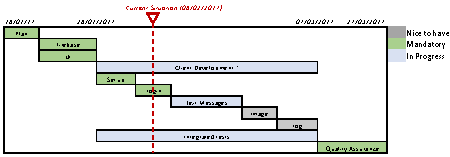
\includegraphics[width=0.9\textwidth]{figs/Timetable}
	\caption{Timetable}
	\label{fig:timetable}
\end{figure}


Please note that our activities in the client development are organized by hierarchy over time. Thus, developing the text message functionality (which is mandatory) is more important than the image message functionality (which is optional but highly desirable). Consequently, we decomposed our activities into tasks and allocated them to each team member as follows:

\begin{figure}[ht]
%[Parzen Window Estimated Distributions]
\centering
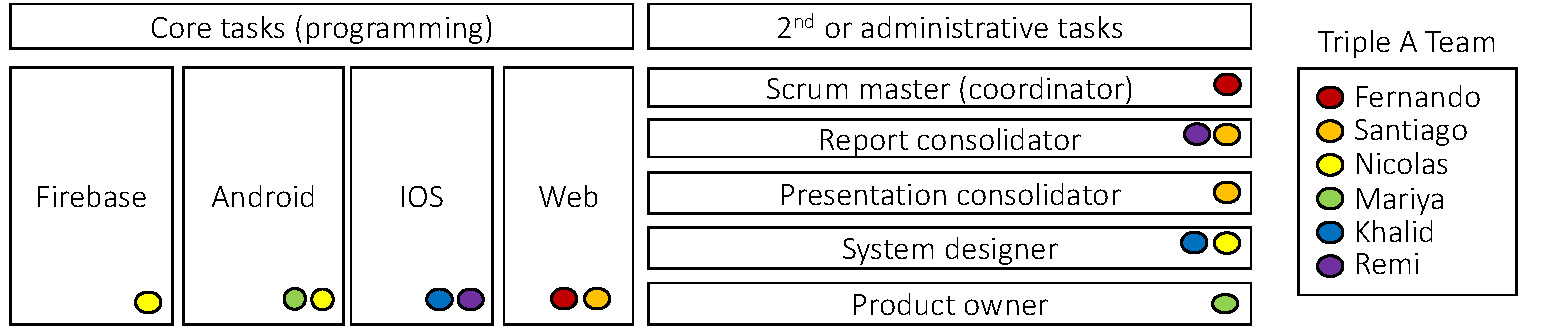
\includegraphics[width=1\textwidth]{figs/tasks}
	\caption{Tasks allocation}
	\label{fig:Tasks}
\end{figure}

\subsection{Current State}
Currently, we have developed the authentication functionality inside the three clients. Firebase authorizes the logged users and allows them see the data only if they are logged in.

\subsection{Next Steps}
Following our timetable, we are going to focus on making the proper database structure (chats, messages, users, receiver, sender, type of message, etc), rules for accessing the data inside the database (only user x and user y can see their own conversation) and adding new data to the database.

\section{Review}
\label{sec:part 2}
Chat applications are around our daily lives. Most of the people don't get out of their homes without checking Facebook Messenger or Whatsapp. Other popular examples, just to mention a few, are chats like Slack, Telegram, Skype, Snapchat and Viber, among many others.

We did research about the most important programming trends and the clients available for the most popular applications. We used Stack Overflow Developer Survey in 2017 ~\cite{DeveloperStackoverflow} as a source, it establishes that the most popular technologies are Android, iOS and Web. In addition, the market share of iOS and Android in 2016 is about 12.9 and 86.2 percent, respectively ~\cite{DeveloperStackoverflow}.  We also added the Web client because web development has always been attractive for us, since companies like Google, Amazon and Facebook started from there. In addition, the entry barrier in a web application is lower than other developing environments.

One of the most important reviews we research at the beginning was proper methodologies to work as a group. Specifically, the agile methodology, proposed by Alistain Cockburn and Jim Highsmith ~\cite{rury346} was our first approach. However, the lack of experience set in and we didn't know how to tackle in advance many of the software challenges laying ahead. Moreover, the proper division of each single task of our software made us struggle at some point, and we  returned to the foundations of the agile methodology. That is, using an hybrid approach on which some tests were conducted at the end and others in each single iteration. In other words, our main challenge in this point was deciding how to tackle each part of the overall system and make the integration. 

As part of the creation of this project, we ultimately decided that in order to get the most out of it, we needed to learn more about different tools. We wanted to pick a challenging technology with the robustness needed but also with vasts amounts of information on the Internet and in books to try and reduce accelerate our learning curve the most we could to mitigate our knowledge lack. 

For the clients we decided to go with Android, iOS and Web and Firebase as our back-end because we were thinking of focusing on the User Experience inside the clients. We wanted users to have a good experience using our service and convince them to use it. From the beginning, we knew that the Authentication is a strong feature in Firebase. It allows us to control who can read your data and also let us select different services such as Facebook, Gmail, GitHub, and others to register and login. One of the main things we found that Firebase has is the real time database. Thanks to this feature, we could see all messages in real time in all the clients. 

As we mentioned before, Firebase was the best choice for our intended purposes, not only because is supported by Google. Aside all the benefits such as Web Analytics, Push Notifications, File storage, and the main reason, the price (which is free for our needs) and also support scalable applications. Firebase gives the flexibility to do a lot of ``back-end" code in the client side. Even though, it leverages a lot to the client, we realised this was interesting to test new ways of developing applications, as we only knew the basics around Object Oriented Programming. It gave us also the flexibility to focus on the front-end development but with the possibility to con troll features that normally a back-end covers. Another of the main reasons why we choose Firebase is that it has a good written documentation on its website. Lastly, it takes minimum setup to begin developing, which was a key point for us as we wanted to finish the project on time while competing between studies and time. Even with this concern in mind we had some challenges finishing it but we have learn a lot in this process.



\section{Requirements, Architecture and Design}
\label{sec:part 3}

\subsection{Requirements}

Table 1 presents our requirements by priority level. Our challenge was to develop as many requirements as we could. We are happy as we manage to develop all the first priority  level requirements. However, we must state that we desired to tackle more of the other requirements set in our priorities but for the challenges we encountered as a team.

\begin{table}[ht]
\caption{Requirements by priority level}
\label{tab:requirements}
    \begin{tabular}[c]{ | p{5cm} | p{5cm} | p{5cm} |}
		\hline
		\centering\textbf{Priority 1} & \centering{\textbf{Priority 2}} & \centering\textbf{Priority 3} &
    \hline
    \parbox[t]{5cm}{-Secure connection\\-Encrypted messages\\ -IOS, Android and Web platforms (at least two platforms)\\ -Contact list\\ -Search for contacts\\ -Sign in by email or Gmail \\ -One to one conversation (text message)} &  \parbox[t]{5cm}{-Send images\\ -Group chat\\ -Chat bubbles instead of username\\ -Notifications of received messages}
& \parbox[t]{5cm}{-Sign in by Facebook\\ -Availability to send other type of media (e.g. video, voice notes, etc.)\\ -Online status of other users\\ -Acknowledgement of received, delivered and read messages, including timestamp\\ -Ability to use the chat offline}\\
    \hline
    \end{tabular}
\end{table}


\subsection{Architecture}

In accordance with the definition of Architecture by Eden and Kazman ~\cite{eden2003architecture}, the next Figure  ~\ref{fig:Architecture}  represents the overview of our design. Thus, we implemented three clients, using Firebase as a back-end, and a JSON, NoSQL (non relational) Database designed to make read operations lighting fast, which involved a trade-off, where we prioritise read speed over data normalisation.

\begin{figure}[ht]
\centering
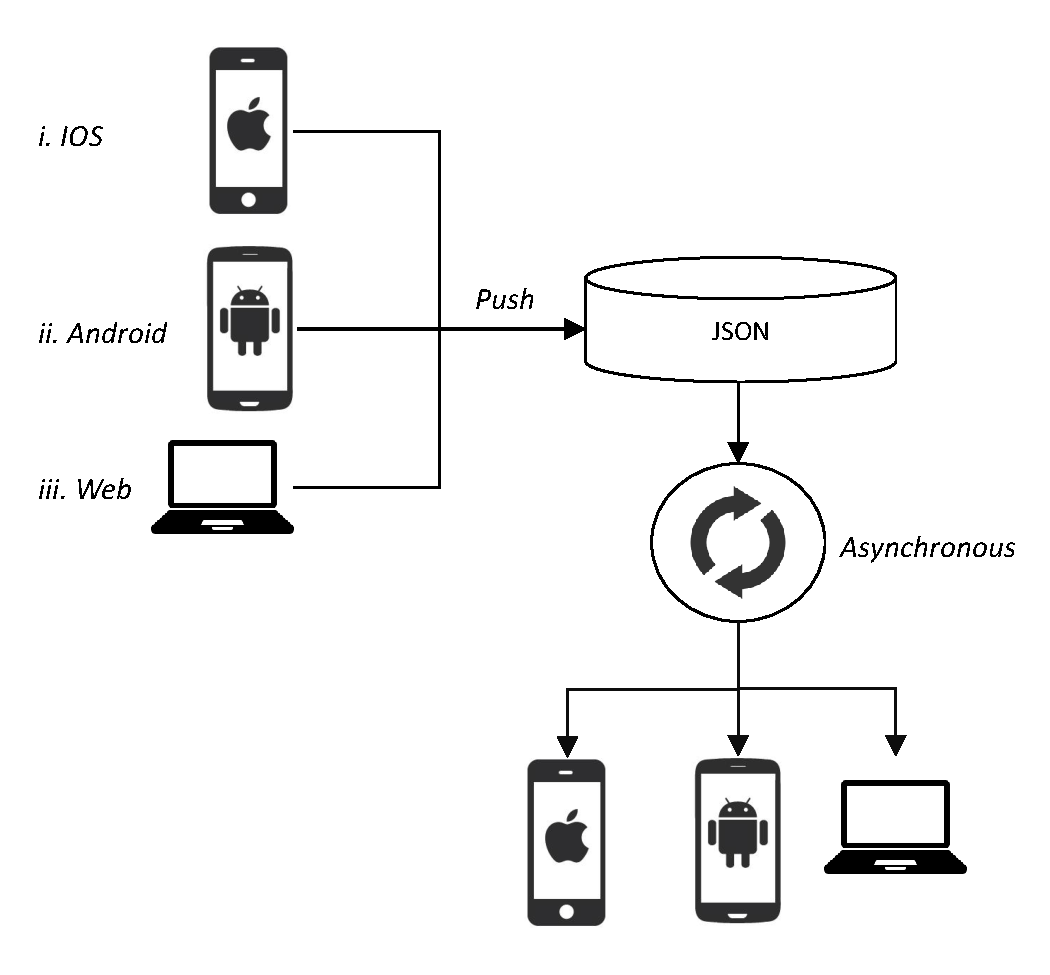
\includegraphics[width=0.6\textwidth]{figs/Architecture}
	\caption{Architecture}
	\label{fig:Architecture}
\end{figure}


\subsection{Database and Back-end}

As earlier stated, we use Firebase as a back-end. This strategy implies to simplify the logic in the back-end and bestow more work to the clients. What we earn by this real fast reading updated than a common design, due to Firebase architecture that provides optimised sockets and a secure protocol.

Firebase consist of a real-time database with an API that allows to synchronise and store data in the cloud with multiple clients. It provides a client library that in our case allows the integration with Android,iOS and Web using Java, Swift and JavaScript respectively. Other services of Firebase as a platform is the storage, hosting (which support static files such as CSS, HTML, media and JavaScript).  To sum-up, Firebase plays a role as a real-time back-end, suitable for scalable applications.

Other interesting characteristic of Firebase is the authentication service, which support social login providers, such as Facebook, GitHub, Google, etc. Another brilliant feature that we used a lot for testing is that we could see in real time the modification of the data. Looking green when new nodes were added, yellow when modified and red when removed. In addition, the crash reporting, as well the analytics tools, caught our attention for two main reasons: i) the possibility to extract information in the future to make more friendly the application (e.g. with performance measures like the average time in the application), and ii) the possibility to test improvements and track changes, with for example A/B tests.

JSON (JavaScript Object Notation) is a lightweight data inter-change format, easier to generate for machines. It is based on i) a set of \textbf{key} and \textbf{value} duple (i.e. an object), and ii) an ordered list of values (i.e. can be string, number, array or even another object) ~\cite{1sejkfhs}. JSON is more lightweight than XML and thus is preferable for web applications because newcomers prefer to handle JSON instead of XML because of the lack of verbosity and readability. Also ~\cite{1sejkfhs} it includes a comparison between the advantages of JSON vs XML.

The following Figure ~\ref{fig:database} presents the structure of the designed database. The idea behind this structure is to prioritise the reading speeds, so messages can be transmitted faster (thus, we duplicate in some cases the data across the tables). That is a strange thing for users that commonly work with relational databases, as a lot of the information tends to be duplicated and not normalised. However, because Firebase is very lightweight, the repetition is not a problem.

\begin{figure}[ht]
\centering
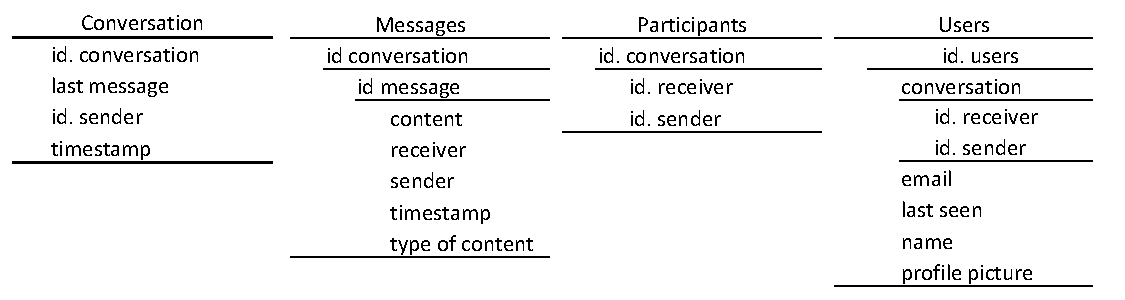
\includegraphics[width=1\textwidth]{figs/database}
	\caption{Database structure}
	\label{fig:database}
\end{figure}

As a comparison exercise, we based our decision starting on a classic design of a relational database, which is showed in Figure ~\ref{fig:rdatabase}. Then, we migrated the design to JSON based on the suggestions that we found online and in the main Firebase docs, this is to optimise its value and allow us to add security and validation rules.

\begin{figure}[ht]
\centering
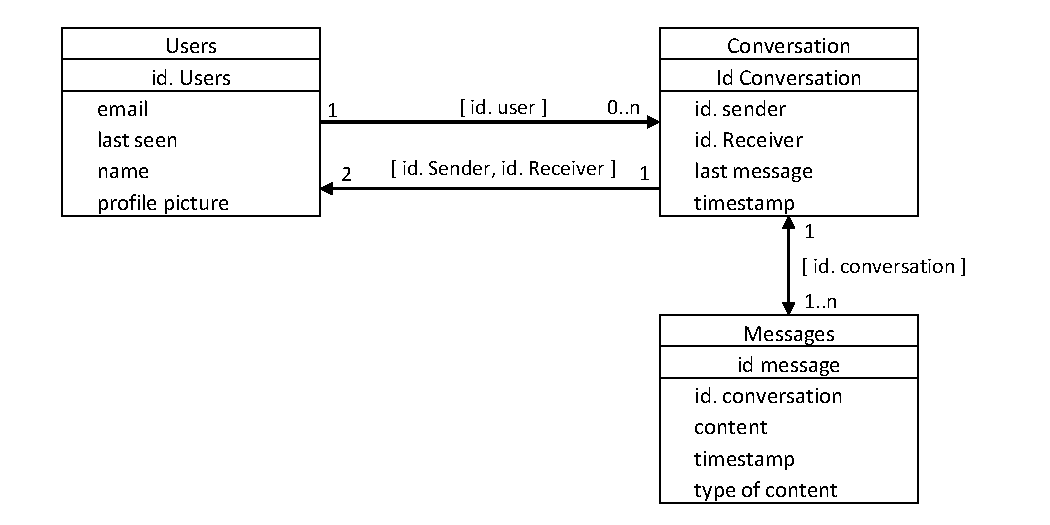
\includegraphics[width=0.9\textwidth]{figs/relationaldatabase}
	\caption{Relational Database initial structure}
	\label{fig:rdatabase}
\end{figure}

The design specified in Figure ~\ref{fig:rdatabase} was also proposed considered the following interaction across the tables, based on three fundamental features: i) sign in, ii) sign up and iii) send messages.  In the case of sign in, the user information last seen field is updated each time. For the Signing up, the \textbf{uid} created by Firebase Auth System is used to create a new user, with the basic information (i.e. id, name, email, and profile picture). Finally, send messages is the most interactive functionality, which works by recovering a conversation id or creating a new id in case there isn't a conversation between two participants available. Furthermore creates a new message which is appended to the respective conversation. To make the query of information easier, the participants table keeps the conversation id, with their respective users id with a value of true in case it exists in that table. We use id.receiver and id.sender for simplicity, however the real sender and receiver properties are shown on the messages dictionary.

\begin{figure}[ht]
\centering
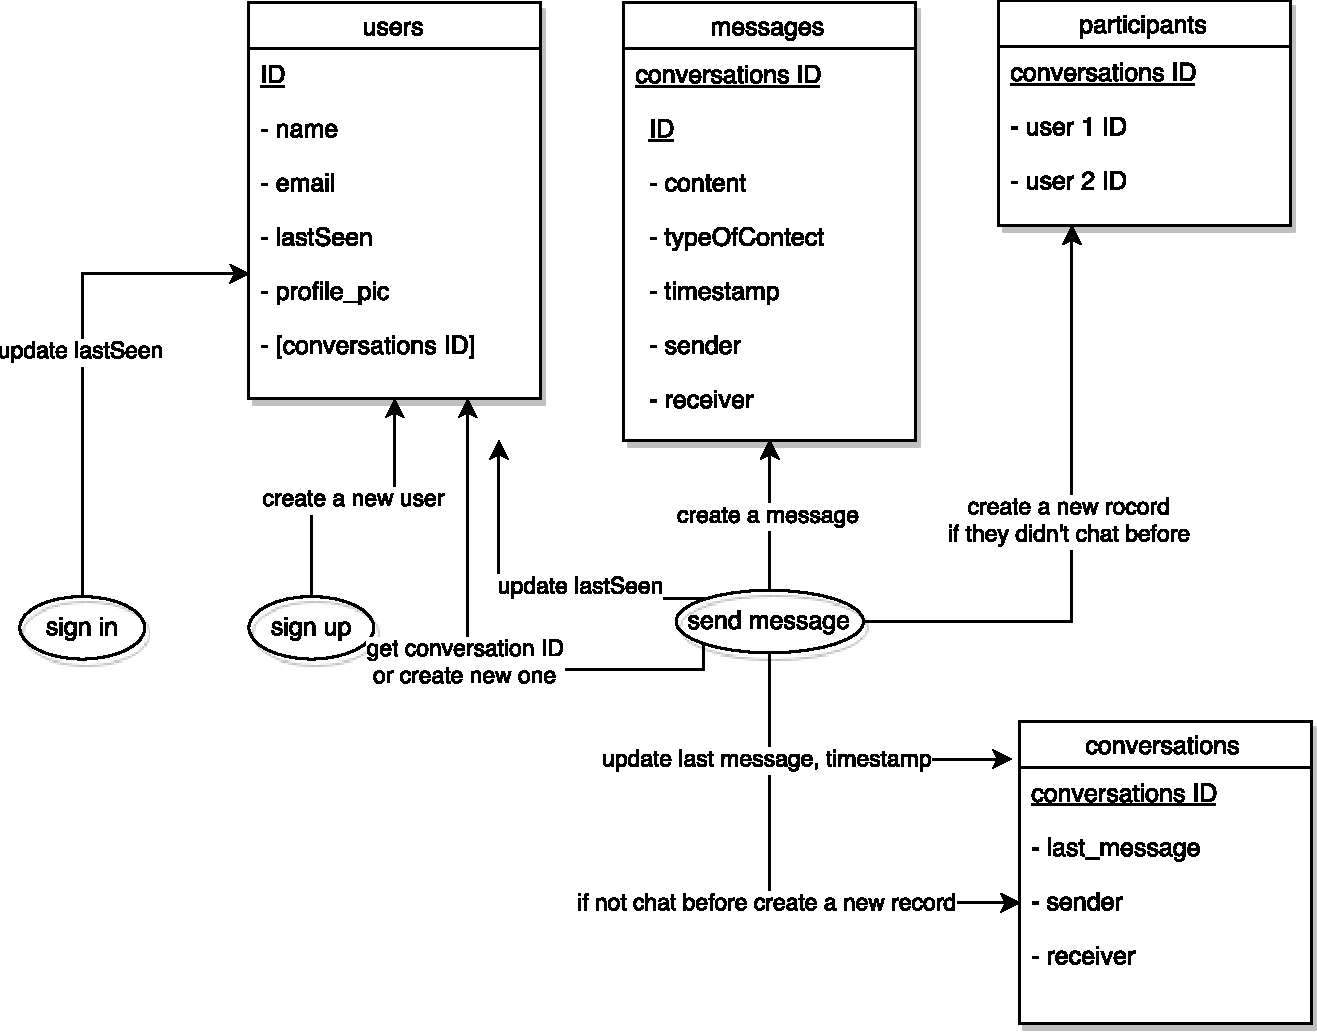
\includegraphics[width=0.8\textwidth]{figs/database_interaction}
	\caption{Database Interactions}
	\label{fig:rdatabaseinter}
\end{figure}


The next section gives more details about the implementation of each specific client. However, the three previously described functionalities and interaction with the database hold for all of them. 


\section{Implementation}
\label{sec:part 4}
This section enters in more details for specifically aspects in the implementation of each client and the back-end.

The next snippet code contains the rule to access the database.  Thus, to read and write in the data base, the authentication process must be succeeded, otherwise is not possible to have access for these two basic functionalities. This is the way to keep suavely the user's information, while security connection is guaranteed with HTPPS through Firebase.

\begin{figure}[ht]
\centering
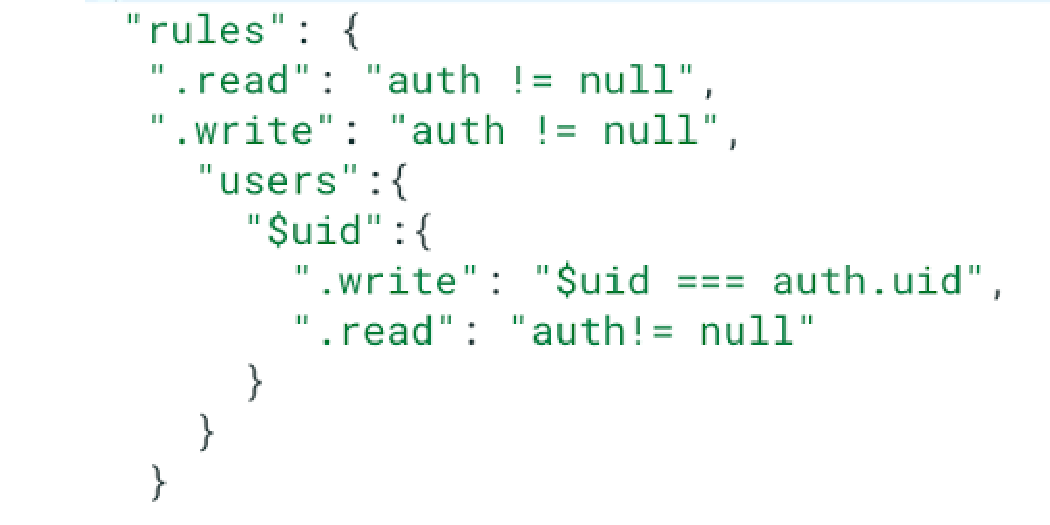
\includegraphics[width=0.5\textwidth]{figs/databaserules}
	\caption{Database Rules}
	\label{fig:databaserules}
\end{figure}

\subsection{iOS Implementation}

Figures 4 and 6 present the specific architecture and database interaction of the iOS client.

\begin{figure}[ht]
\centering
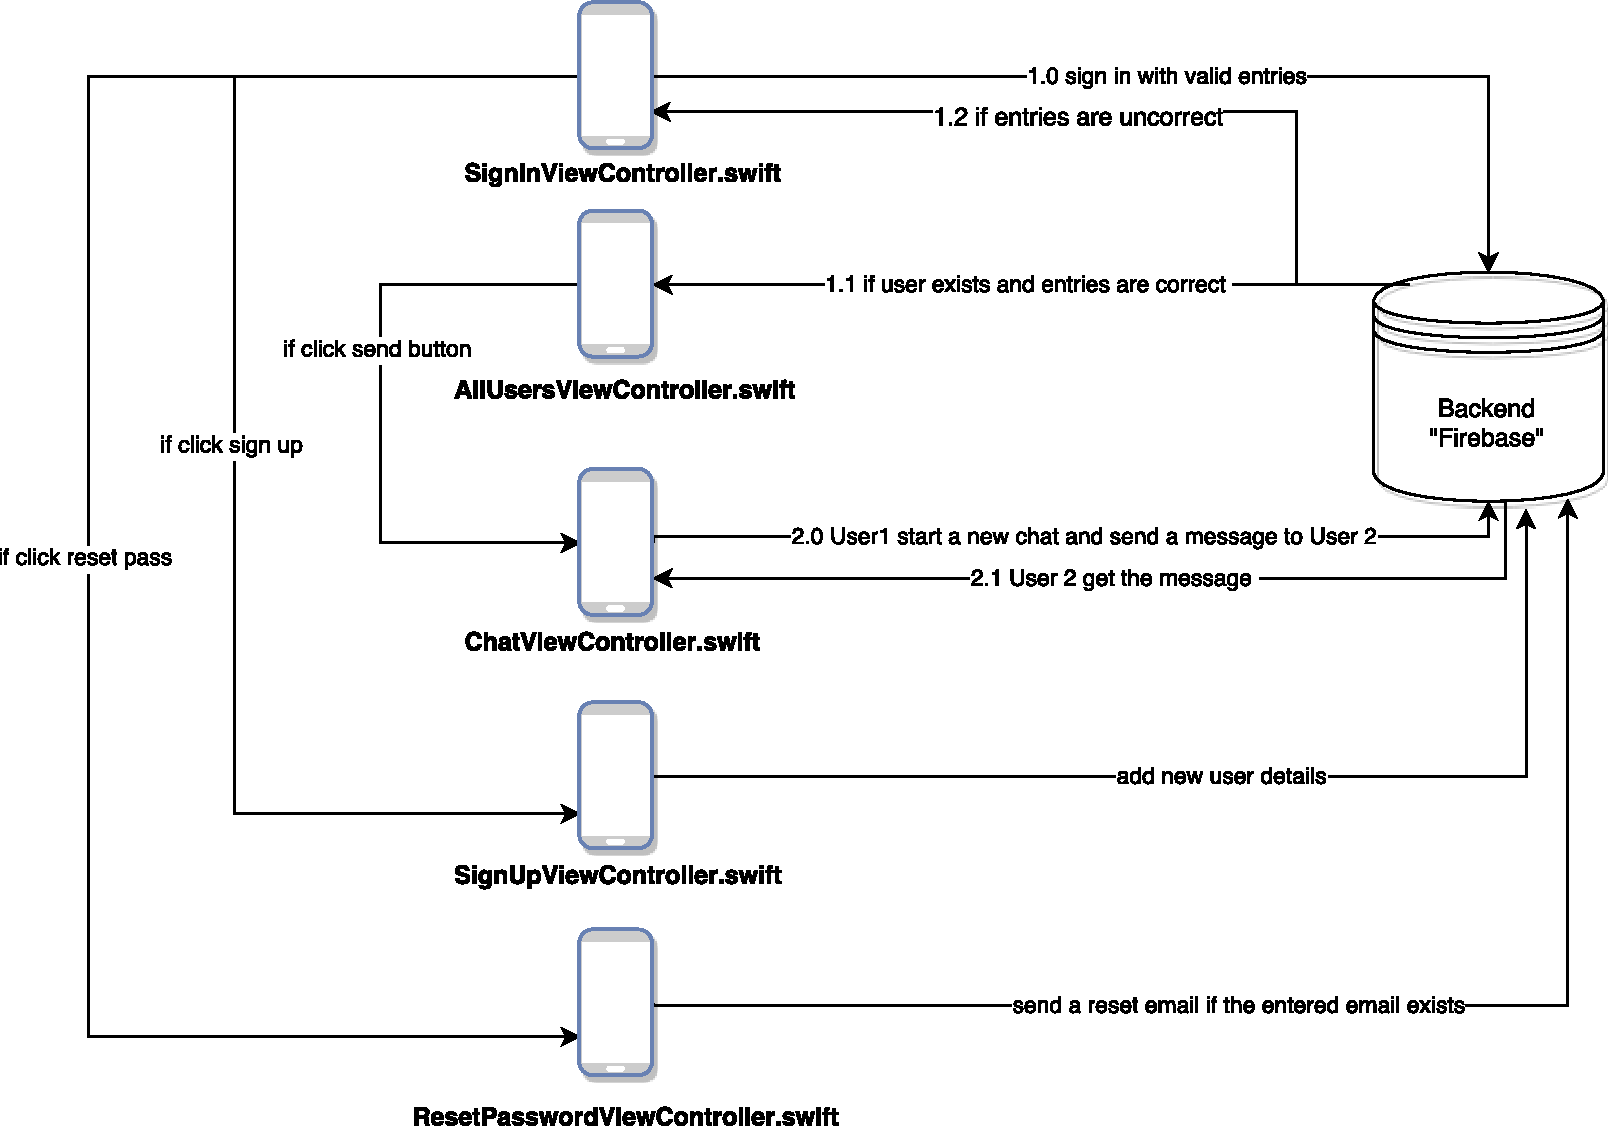
\includegraphics[width=1\textwidth]{figs/iOSarchitecture}
	\caption{iOS Database Interactions}
	\label{fig:iOSarchitecture}
\end{figure}
\textbf{Achievements and Challenges}: The iOS client was able to carry out all the tasks listed under Priority 1 successfully. We were able to achieve secure connection, messages, contact list, sign in by email, one to one conversation across the platforms. However, some of the most challenging aspects were how to fetch users and check if the users have chatted before. Some of the most relevant specific details across iOS development are also stated in the next subsections while some screen-shots of the GUI are in Figure 16. 

\begin{figure}[ht]
\centering
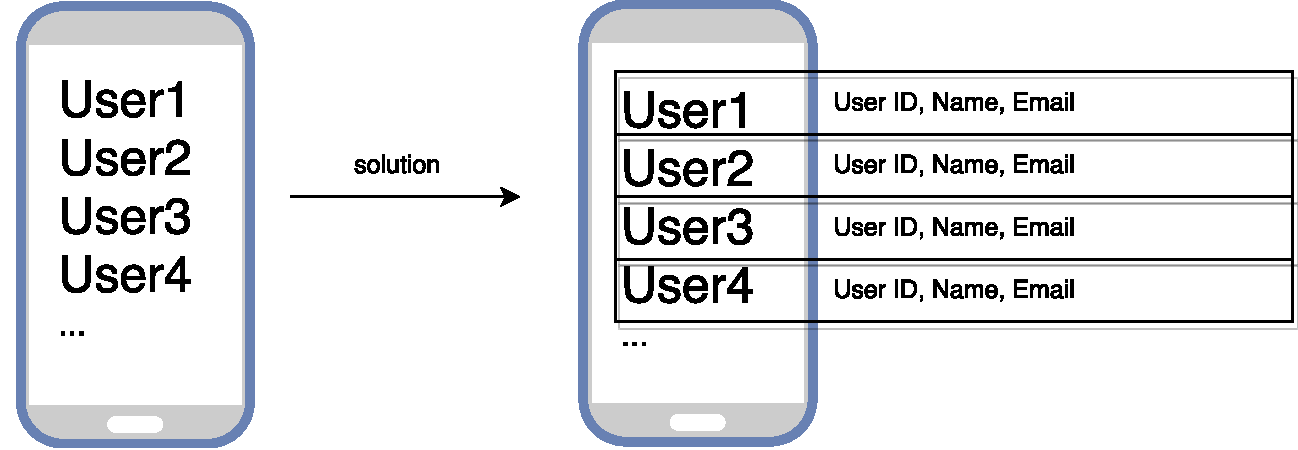
\includegraphics[width=0.75\textwidth]{figs/iOS_fetch_users_ID_issue_and_solution}
	\caption{Fetching Users in iOS}
	\label{fig:iOS_fetch_users_ID_issue_and_solution}
\end{figure}
  

\textbf{Fetch users}: The sender must ensure that the sent message go only to the intended receiver using the first UI (left side in Figure 7). To resolve this, we fetch the data of users as an array of array (as shown in the UI on the right of Figure 7) from the back-end to have the ID of the selected user.

\begin{figure}[ht]
\centering
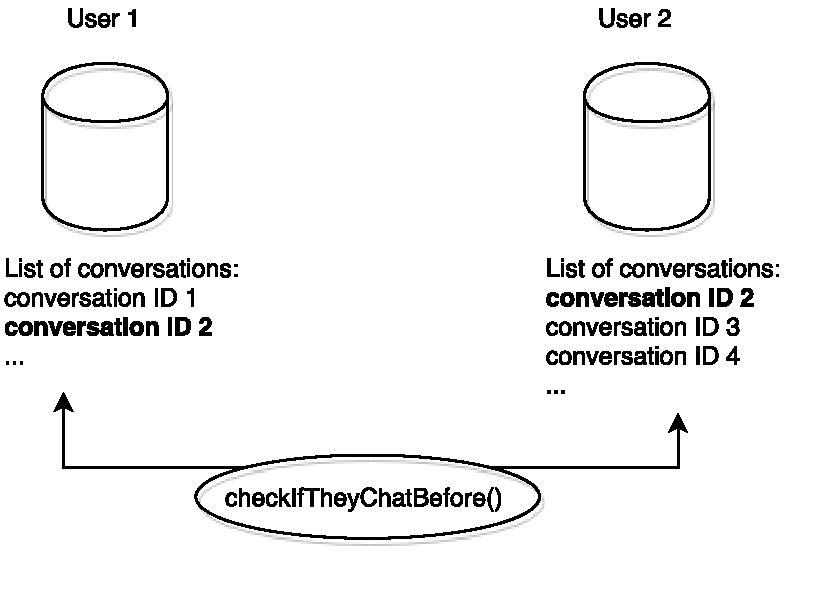
\includegraphics[width=0.6\textwidth]{figs/iOS_check_if_they_chatted_before}
	\caption{Helper function to check if chat exists}
	\label{fig:iOS_check_if_they_chatted_before}
\end{figure}

\textbf{Check if they chatted before}: When the user is trying to set up a new chat, it was difficult to find out if there is a previous chat with the receiver. There were several attempts made using different approaches to figure out a solution. Finally, we were able to come up with a function that carries out the logic shown in Figure ~\ref{fig:iOS_check_if_they_chatted_before}). Once a user (User1) selects another user (User2) to chat with, the function checkIfTheyChatBefore() compares the IDs of conversations from both sender and receiver records.  If there exist a common ID, then it implies that they had chatted before and the same conversation ID is used to store messages. Otherwise, a new conversation is created in the database.

\textbf{External Library}: We used two libraries namely; UIKit and CocoaPods. UIKit is a library already integrated in xCode which was used to make text fields, buttons, labels, and tables. However, using Cocoa Pods is mandatory for Firebase as a back-end.

\textbf{Code by others}: We use a code written by @Esqarrouth from http://stackoverflow.com/ to write the function hideKeyboardWhenTappedAround() in SharedFunc.swift (Github: Whisper/iOS/iOS/) which hide the keyboard when user taps anything else on the screen other than the keyboard.

\subsection{Web Implementation}

The WhatsApp Web Client was a great inspiration for us. Some of the key aspects of our web app are as follows. For the registration, we use a small plug-in called FirebaseUI that helps us connect with Firebase and select the providers we want to choose. We used Mail, Google and Facebook because those are the most popular.

For the whole App Wrapper, we used React JS which is a JavaScript Library developed by Facebook. React basically works as a multi component oriented framework that aims to simplify the logic of web applications by making apps more modular. It handles all the information, including user interface state in a state object that can be shared with other components or a local state only available to itself. After some event occurs, react re-renders the changed component to reflect the new state. Along with it, we learn the hard way that a Chat application needs a lot of rendering of elements in both direction (from parent to children and backwards). Therefore, we struggled a lot and we changed our main objective by doing some research and finding out that precisely, a lot of developers had the same problem when dealing with these type of applications. They were communicating bidirectionally between parents and children in the DOM Tree way too many times. That's how we learnt that Whisper was an excellent use case for Redux. 

Redux is another library that dispatches actions from the user interface to a reducer, which in turn sends the new state to the store (which is a global state for the app). Also with this, we learned the hard way that Redux couldn't manage asynchronous calls to a server by itself. Therefore, we used a middleware called Redux-thunk which takes care of this by simply dispatching actions on demand. That is, dispatch an action when we finished, for instance, fetching elements from Firebase.

Finally, for the styling we used stylus, CSS, and Bootstrap alpha 4 to accelerate our development and learn the newest trends in the front-end development community.

It is important to mention that we learned a lot of web development thanks to this project. We focused in these technologies because they are among the most used online in communities like Stack Overflow, Hacker News, and Reddit Web Development related subreddits.

Contrasting with iOS and Android, there are so many options out there to begin Web App Development. Being objectively, HTML and CSS are just not enough for this kind of project. As we know, HTML only serves the purpose of giving the structure to the web. That is, structuring all the information inside the DOM hierarchically and in order, tag by tag and element by element. As the name suggests CSS (Cascading Style Sheets), give the style or appearance to each HTML tag inside the DOM, properties such as position, colour, font weight, variant and sizes, background images, padding, margin, etc., are the ones that CSS controls so users can have a much better experience. 

However, we knew that this project was going to be heavy on the scripting side; we started looking out for technologies to take our development to the next level. Some of our research suggested that we used a powerful framework that took care of the rendering of elements almost in real time. To take advantages of the asynchronous functionality of Firebase, we decided to try it with the following various contestants: Vanilla JavaScript, AngularJS, ReactJS, jQuery and Ember.

Pure JavaScript is always needed for every heavy front-end development app, because that's the scripting part of it. However, pure JavaScript can lead to messy code and just recently with ES6 and ES7, with modular exports, is getting more friendly towards heavy applications, as we know. Although we are not experts at all and some of us have a little bit more experience using Python and Django for Back-End software development, we see a lot of resemblance between JavaScript classes and exports with Django Class Views.

AngularJS was an attractive option, is powered by Google and we consider this as a plus. Also, there are tons of material out there to learn, from community blog posts and books to complete courses on Coursera. On the other hand, jQuery is a JavaScript Library that has been out there since 2006, and although front-end frameworks change continuously  ~\ref{fig:5656rtyrt}, we learnt that jQuery was a leader at the time and still, for some basic stuff like AJAX is the go to for full-stack developers. 

React, being developed by Facebook, has a really strong community and hype around Internet blogs and the Stack Overflow Community Survey of 2017 ~\ref{fig:DeveloperStackoverflow}, however we didn't knew the potential until we read the well written documentation of it.

React's documentation, ease of use and hype, gave us the confidence to pick it up as a great library/framework to learn from. That's why we choose it for the Web Client development. React is used mainly by experienced software engineers in the front-end development industry. React facilitates most of the job on front-end development because it suggests to create your web applications using components for each task that needs to be done by your app, however that doesn't make it easy. Treating every bit of it as an isolated component that can even be reused on different future apps is the main benefit against others. The scope of these components is to focus on doing an specific task to make your application easier to understand to other developers. 

React is a little bit intimidating, some of the information out there can be confusing because to develop for it you need a little extra setup. Not like iOS or Android which only need Xcode and Android Studio respectively.

In contrast, you need to install NodeJS, npm (included) and Babel to transpose JavaScript newest syntax for older browsers. Additionally, they always suggest to use Gulp or Grunt to create tasks that automate a lot of the repetitive and tedious tasks inside front-end development such as compiling the different JavaScript source files, merging together all the CSS or style files, and running web pack to refresh your website with hot reloading whenever a new change is detected (basically to avoid refreshing the browser window).

All these tools that we have just mentioned are just needed for the development. For the actual code to make its job and suggested by React inside their documentation, they advise to use JSX, which is basically a way of writing JavaScript and HTML inside your JavaScript files.


\begin{figure}[ht]
\centering
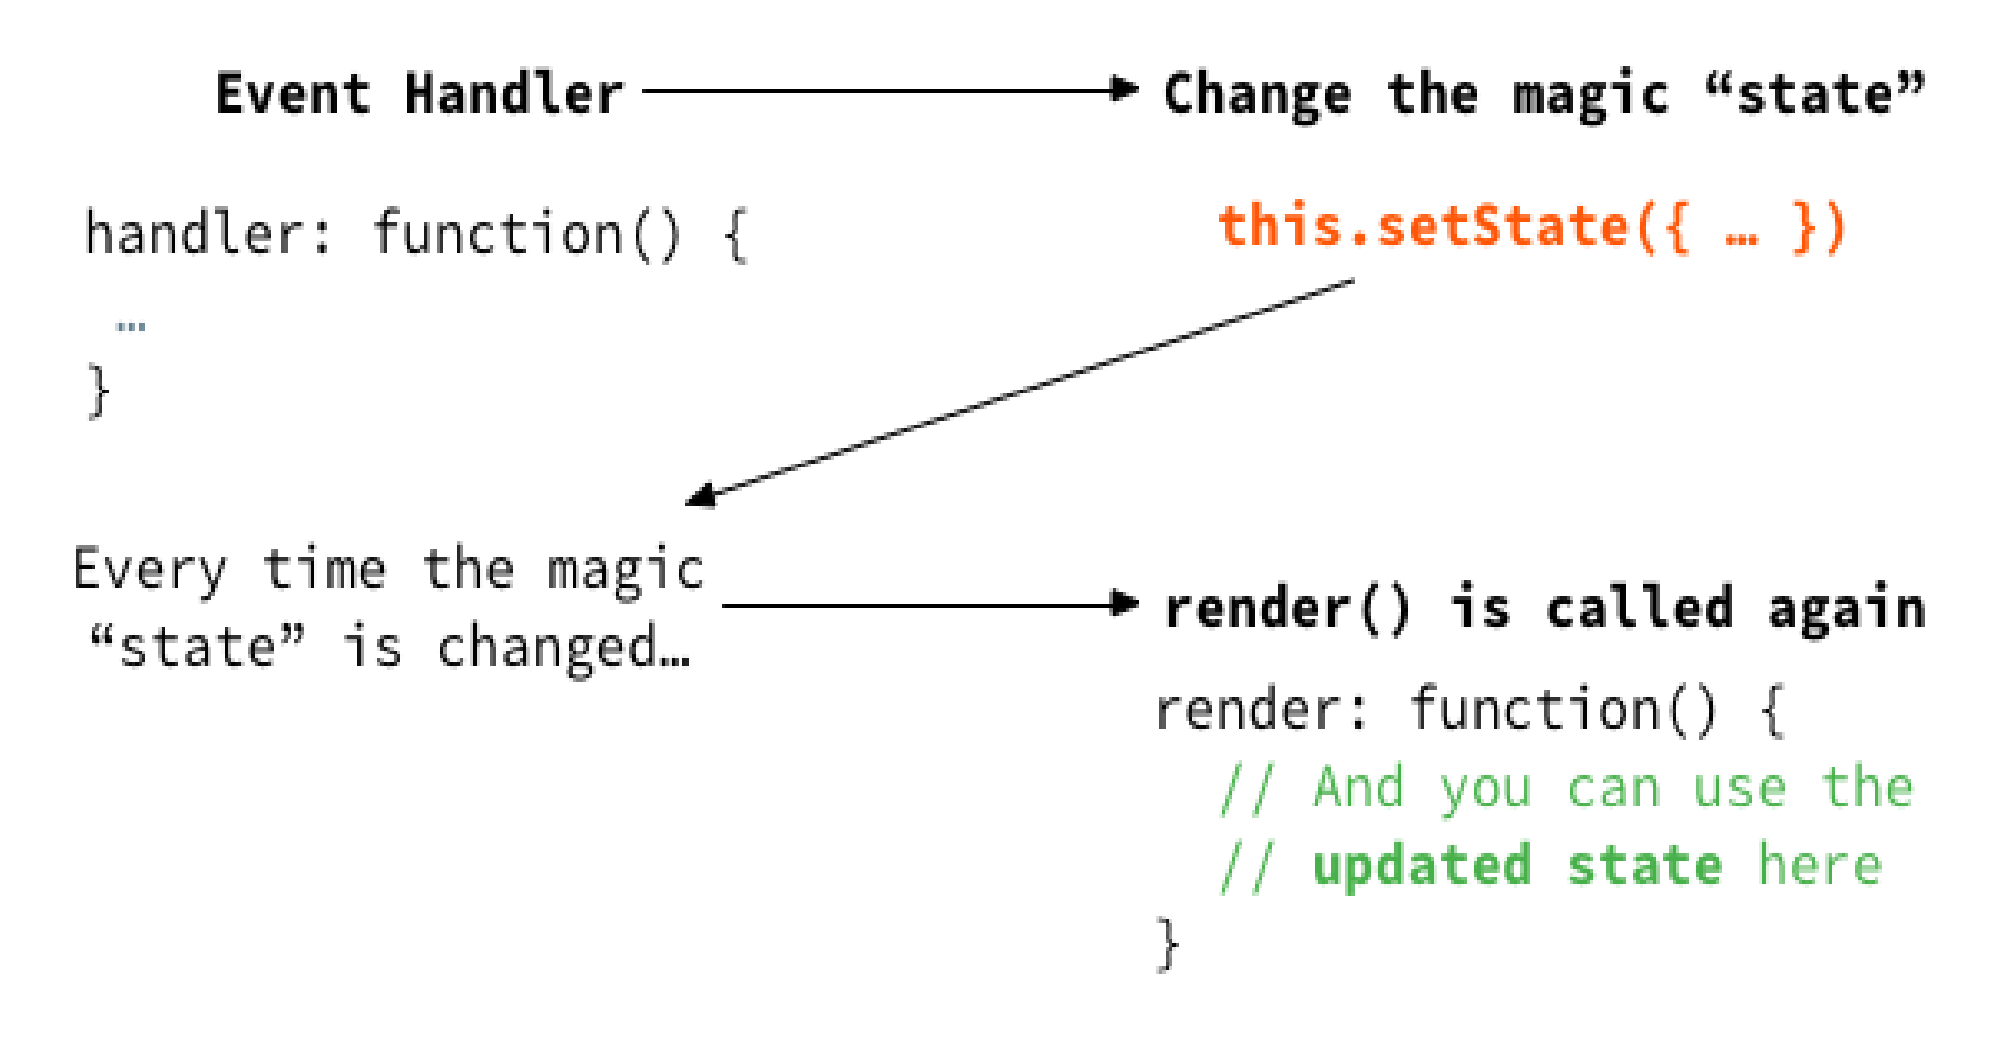
\includegraphics[width=0.6\textwidth]{figs/reactstyle}
	\caption{Overview React State and Render}
	\label{fig:reactstyle}
\end{figure}

Modular components and state are the most important aspects behind React development. For our case, it was very useful because our code was structured this way to achieve way more readability (on most of the cases) and to think about the big picture easily. And state management was very helpful because we could see state in real time thanks to the Chrome React extension. By this, the debugging process is less painful and much more friendly.

Some aspects of JavaScript language specifically made us struggle a lot, mainly because we did not have enough experience but mostly because of the ES5/ES6/ES7 standards and the way some documentation refer to their best-practices. That is why many people suggest using a library called Babel which was created by one of Facebook's employee ~\cite{4646eyyeye}.

This library, among other capabilities, gives the developer the ability of using fat arrow functions and in general features that are not yet available in some browsers:

\begin{figure}[ht]
\centering
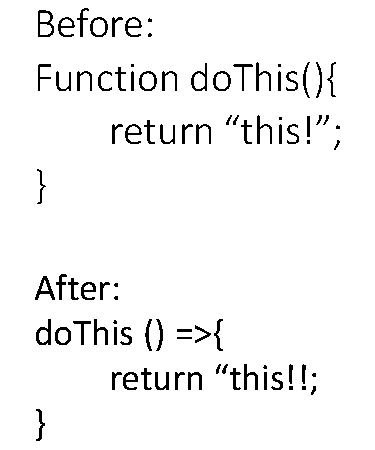
\includegraphics[width=0.2\textwidth]{figs/before}
	\caption{Fat Arrow Functions in JS}
	\label{fig:before}
\end{figure}

Some of these features of the JavaScript programming language gave us difficulties. One problem that really complicated things was the “this” keyword in our functions. Apparently in JavaScript this is not the same as, for example, “self” keyword in Python. More on that later when we explain Firebase integration.

In React, we opted to have the following main components which can be found inside the components directory:



\begin{enumerate}
	\item \textbf{AppWrapper}: The whole container wrapping all the components together and passing the state from Redux (more on that below) to the rest of the components.
	\item \textbf{ConversationsSidebar}: To render on the left side of the app, the conversations that each user have.
	\item \textbf{ConversationPanel}: The right-side panel that shows all the messages sent between users inside the selected conversation of the ConversationSidebar.
	\item \textbf{UserDrawer}: In charge of showing all the users available inside our application in the Users JSON (except the current logged user).
	\item \textbf{AddMessage}: This is the main component that takes care of dispatching most of the logic whenever is triggered. This is the main form element that adds the message to the Messages, Conversations, and Participants JSON when needed.
					
\end{enumerate}


We used Redux, because at first we tried it the hard way. We were using pure React to develop our app but because in react you must pass all the state from the parents all the way through the children that needs that piece of state, code can get chaotic. The following image illustrates how Redux solves a lot of the passing props from one side to another by using an independent store that handles all the data.

\begin{figure}[ht]
\centering
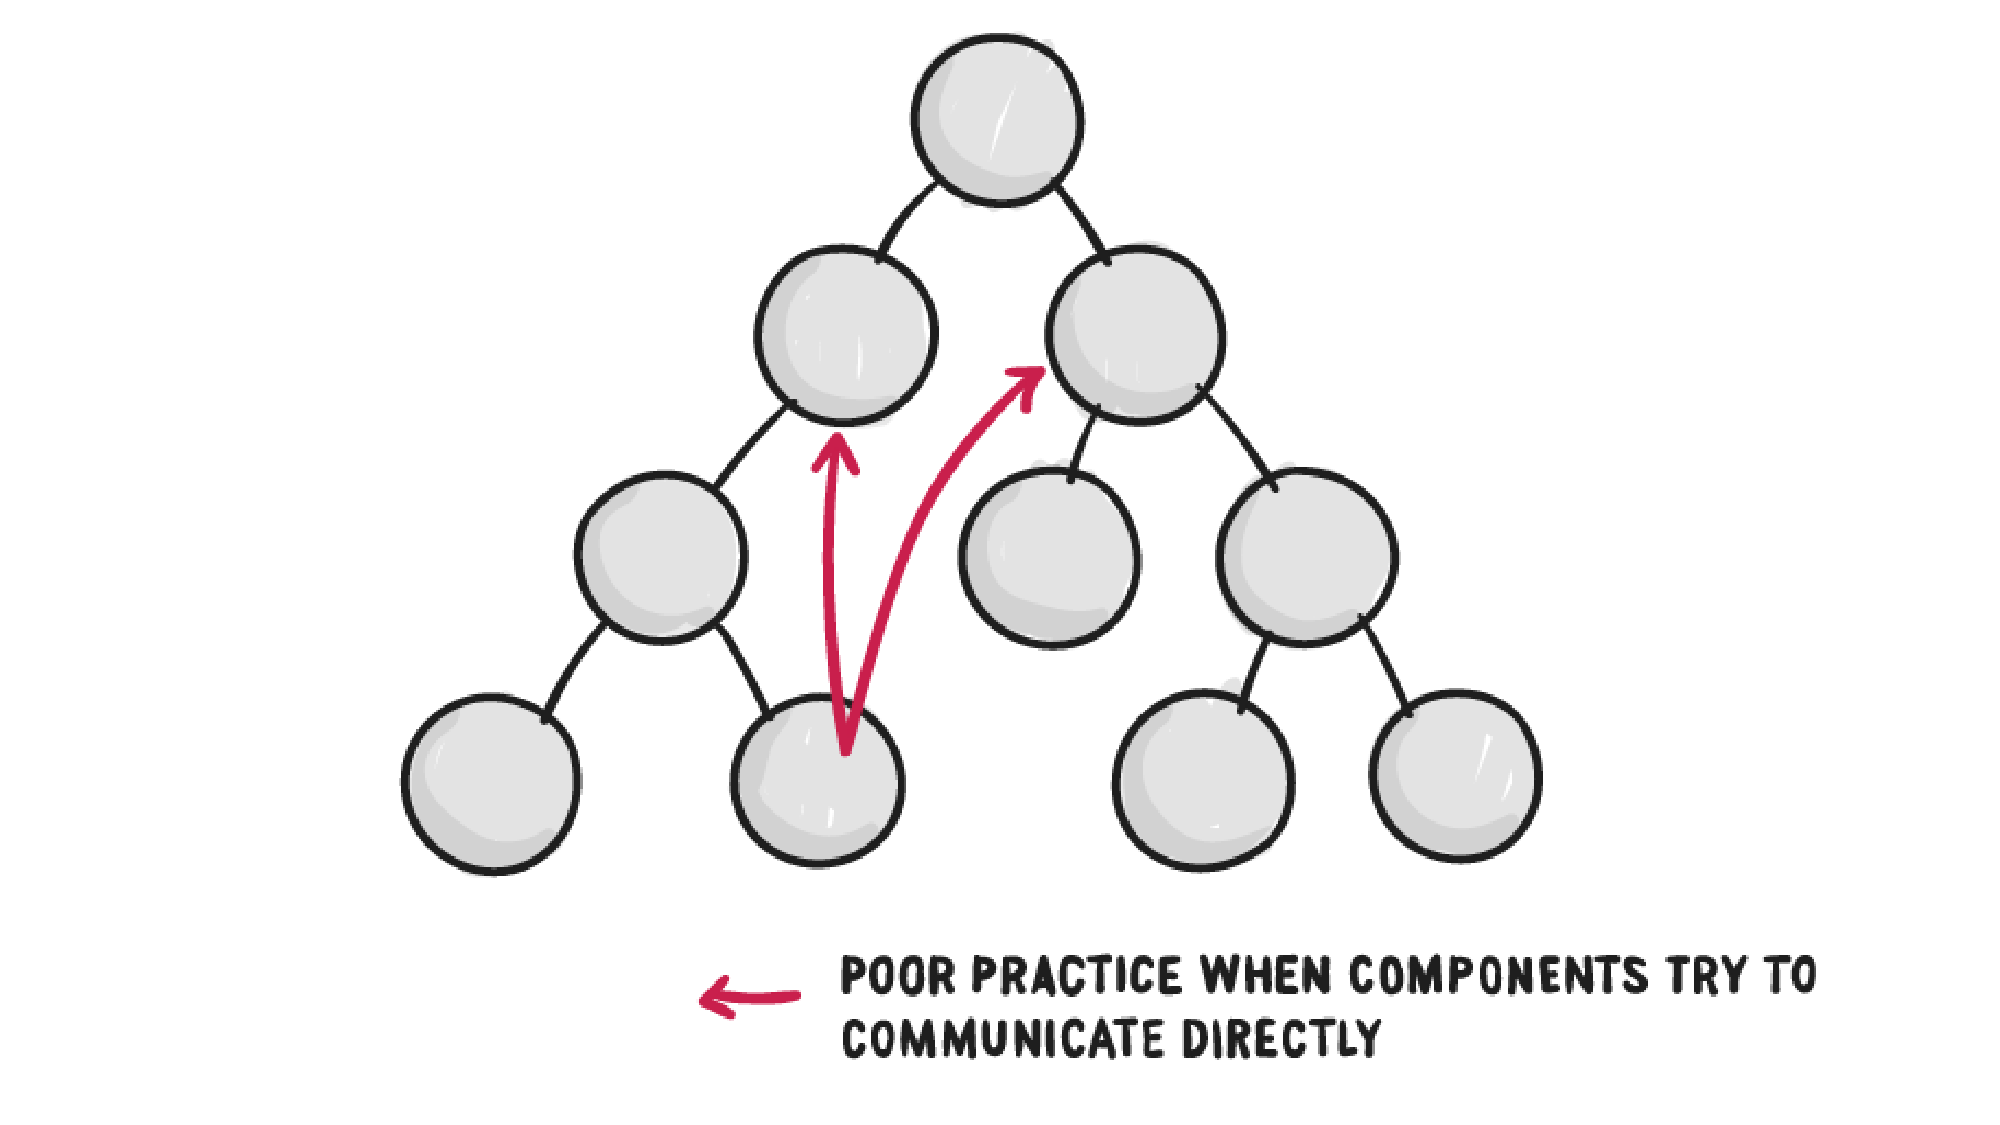
\includegraphics[width=0.5\textwidth]{figs/poorpractice}
	\caption{Hard to do when app gets complex}
	\label{fig:poorpractice}
\end{figure}


\begin{figure}[ht]
\centering
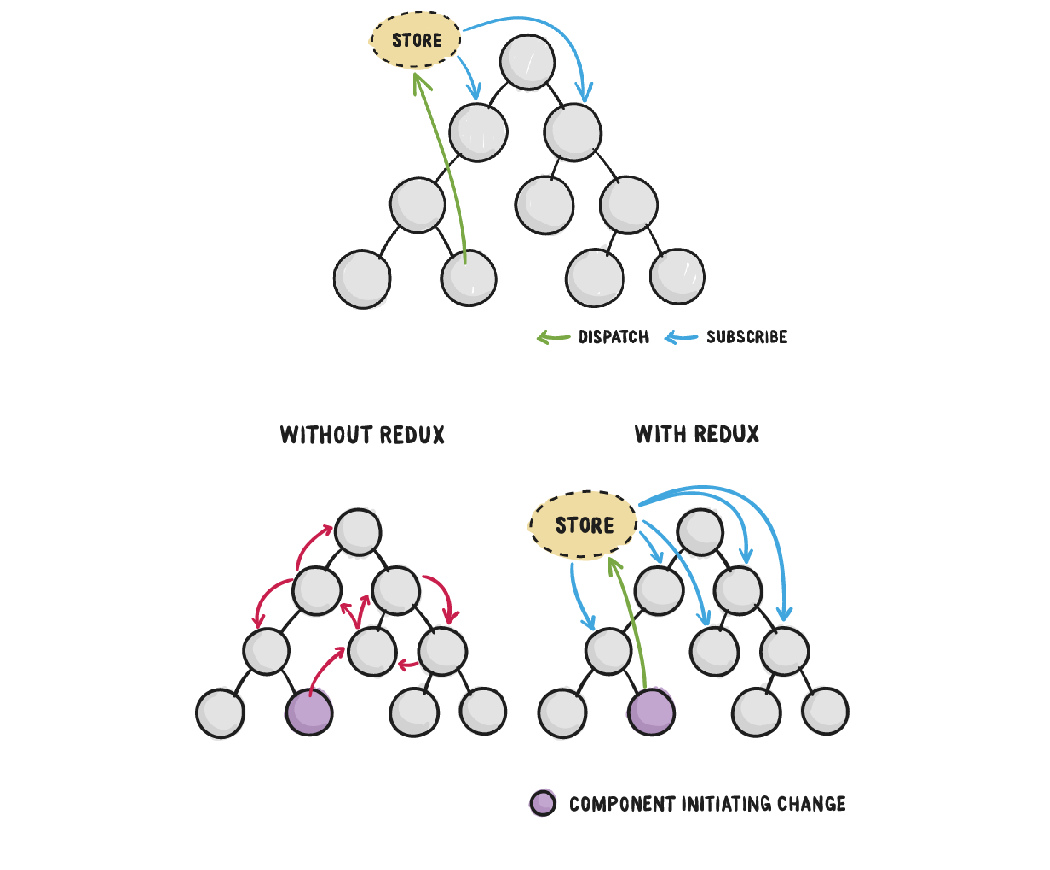
\includegraphics[width=0.5\textwidth]{figs/rtrtrtryeyeyeye}
	\caption{How Redux solves this}
	\label{fig:rtrtrtryeyeyeye}
\end{figure}

We were advancing with the application when we realised that code started to get complicated. That’s why in our commit history we show a drastic change of code from non Redux to it.
Using Redux was not as easy as we thought. The theory behind it is simple, use a store that holds all your app state (conversations, users, messages, and participants), fill that state when needed by using Actions and Dispatchers and then return the modified state with the Reducers.
Actions is a very simple concept, every time something happens in the client, an action is dispatched. When this action is dispatched, all the reducers listen, if they “own” the given action, then they update the state accordingly. One of the most important parts of Redux is that Reducers need to be pure functions.
The whole state of your app is stored in an object tree inside a single store.
The only way to change the state tree is to emit an action, an object describing what happened. We write reducers to specify how the actions transform the state tree ~\cite{ryryyrt346}.

Pure functions mean that you should not mutate the state object, but return a new object if the state changes. This is tricky at first and we ended up making a lot of mistakes on the first implementation, however, React and Redux documentation explain it well, however we didn't understand it. Which resulted in these errors of strange behaviour between state changes.

All our logic for Reducers was added to a folder called Reducers. The same thing for Actions, all are inside the actionCreator.js and the Constants for it are on the file with the same name.

The next Figure ~\ref{fig:actions-states} explains how our Whisper Web Client handles actions and state.


\begin{figure}[ht]
\centering
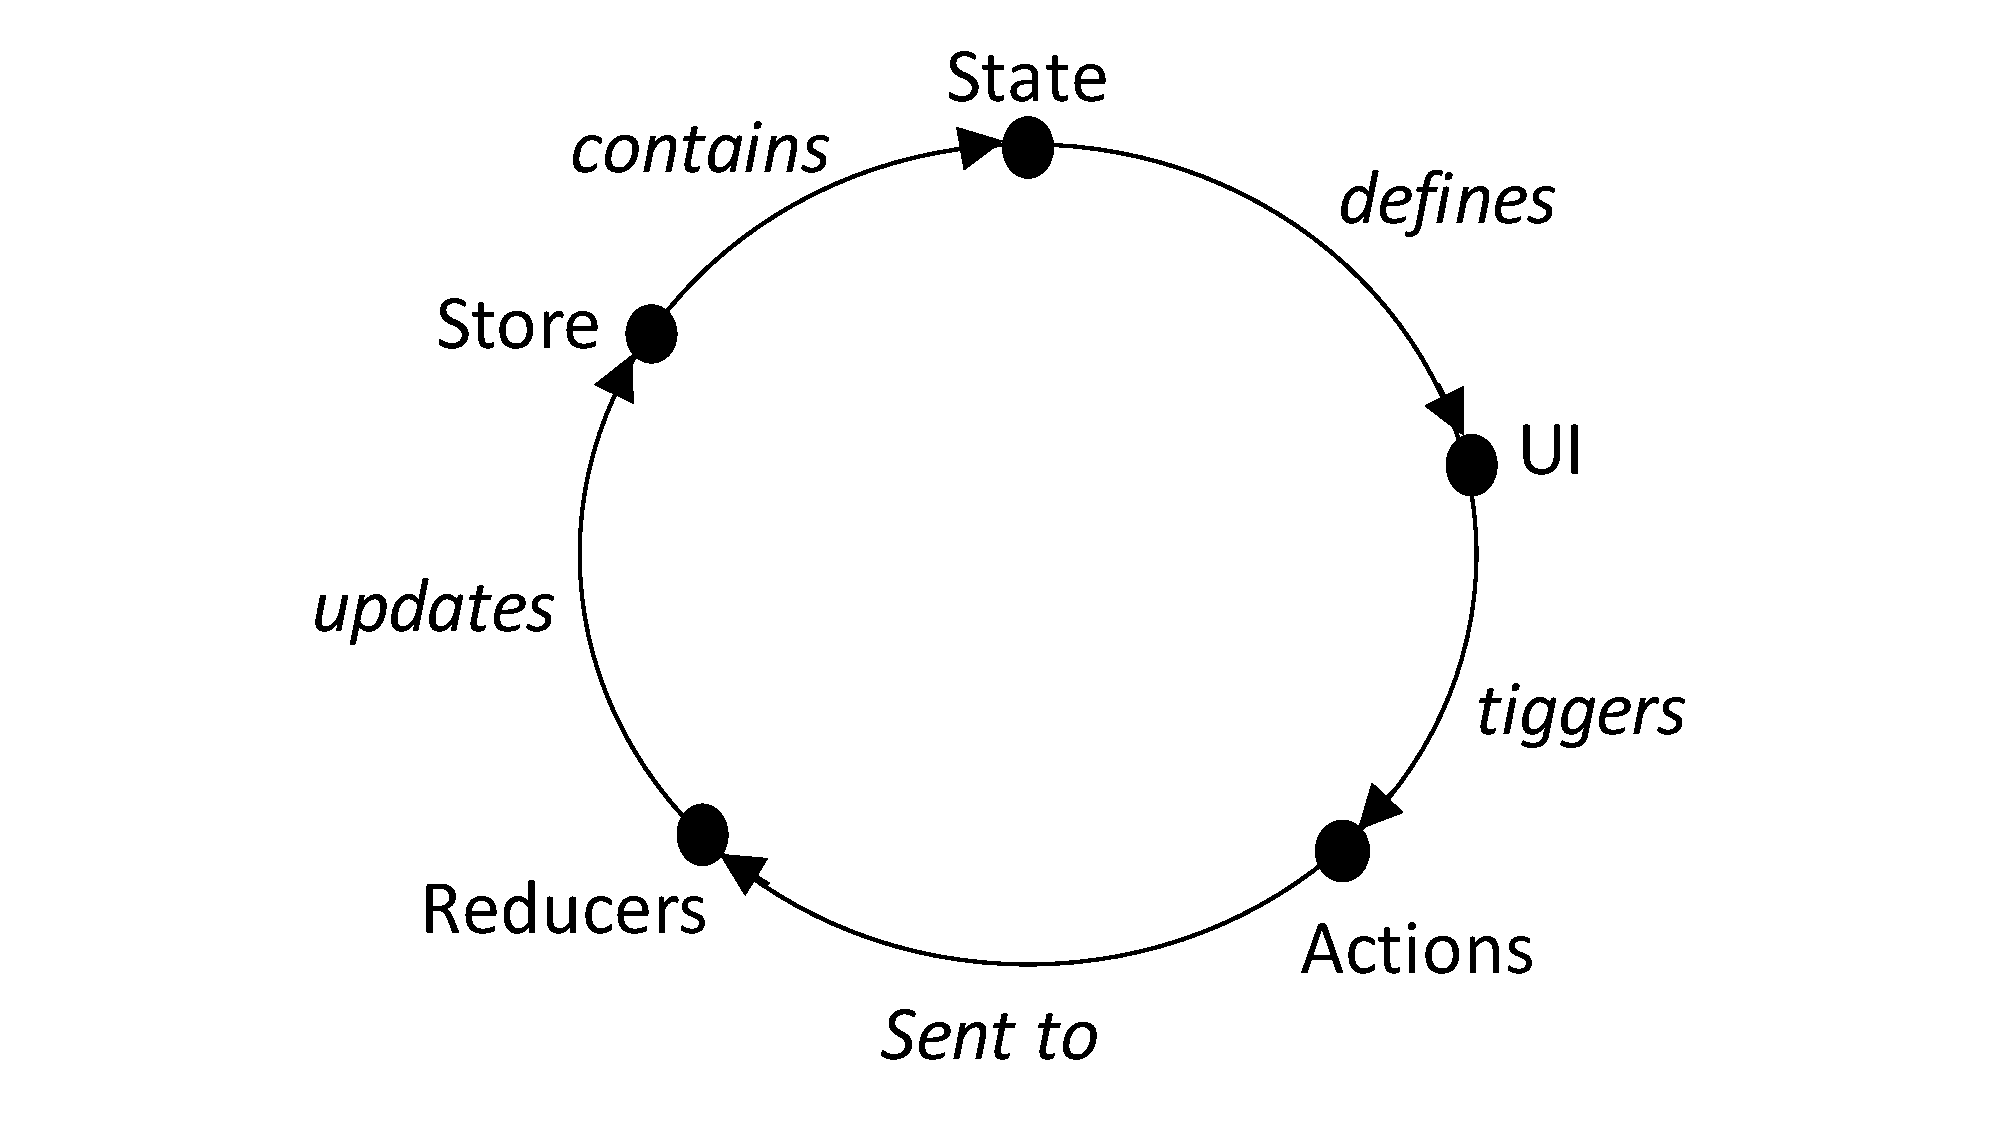
\includegraphics[width=0.5\textwidth]{figs/actions-states}
	\caption{Web client actions and states cycle}
	\label{fig:actions-states}
\end{figure}


Integrating Firebase was one of the most complex tasks because even though the documentation is excellent, there is not enough information on how to integrate Firebase with React and Redux. When we started, our app using only React, everything was handled by functions inside the components. However, because of Redux nature of pure functions Asynchronous calls where a struggle for us. That's why we needed to add a middleware called Redux-thunk ~\cite{46rtrtet}. This is another library widely used by the React Community. However, there is also another one gaining popularity called Redux-saga ~\cite{5656ry} which solves the same issues, doing asynchronous calls inside Redux, that is, fetch and update Firebase whenever an action is dispatched via Redux.

Previously we mentioned how we needed to use Babel to compile our code because of the new Arrow Functions and the \textit{this} keyword. With Firebase, some of the methods didn't work as expected inside React. After much research, we finally found an explanation of this behaviour on StackOverflow which told us that with React and Firebase you had to either “bind” this keyword or use a fat arrow which does this automatically for you. At first the arrow function looked intimidating, but it was less boilerplate code for the rest of the app, so we decided to use this newer feature inside JavaScript and fix the babelrc file accordingly. 

Once we got this issue solved we got on speed, we were getting all the information from Firebase as we needed. The first part was fetching the conversations from Firebase. We used some sample data following the structure we mentioned before. With Firebase, we fetched all the conversations that the loggedUser had in their conversations object. This was one of the most important highlights of our project, because as opposed to a regular SQL Database, there is no such thing as “SELECT * FROM Conversations where conversationID in (SELECT Conversations FROM User WHERE User = “X”)” With Firebase we had first to read the loggedUser, which by that time was a hard-coded “uid” which is the Id that Firebase gives to every new registered user. After that, we needed to fetch all the conversations from that User. And when we finally got those conversations in the same step we needed to fetch all of to the Conversations of the Conversation reference object that were the same as the User’s. This code was really hard to achieve, so we are really proud we got it:


\begin{figure}[ht]
\centering
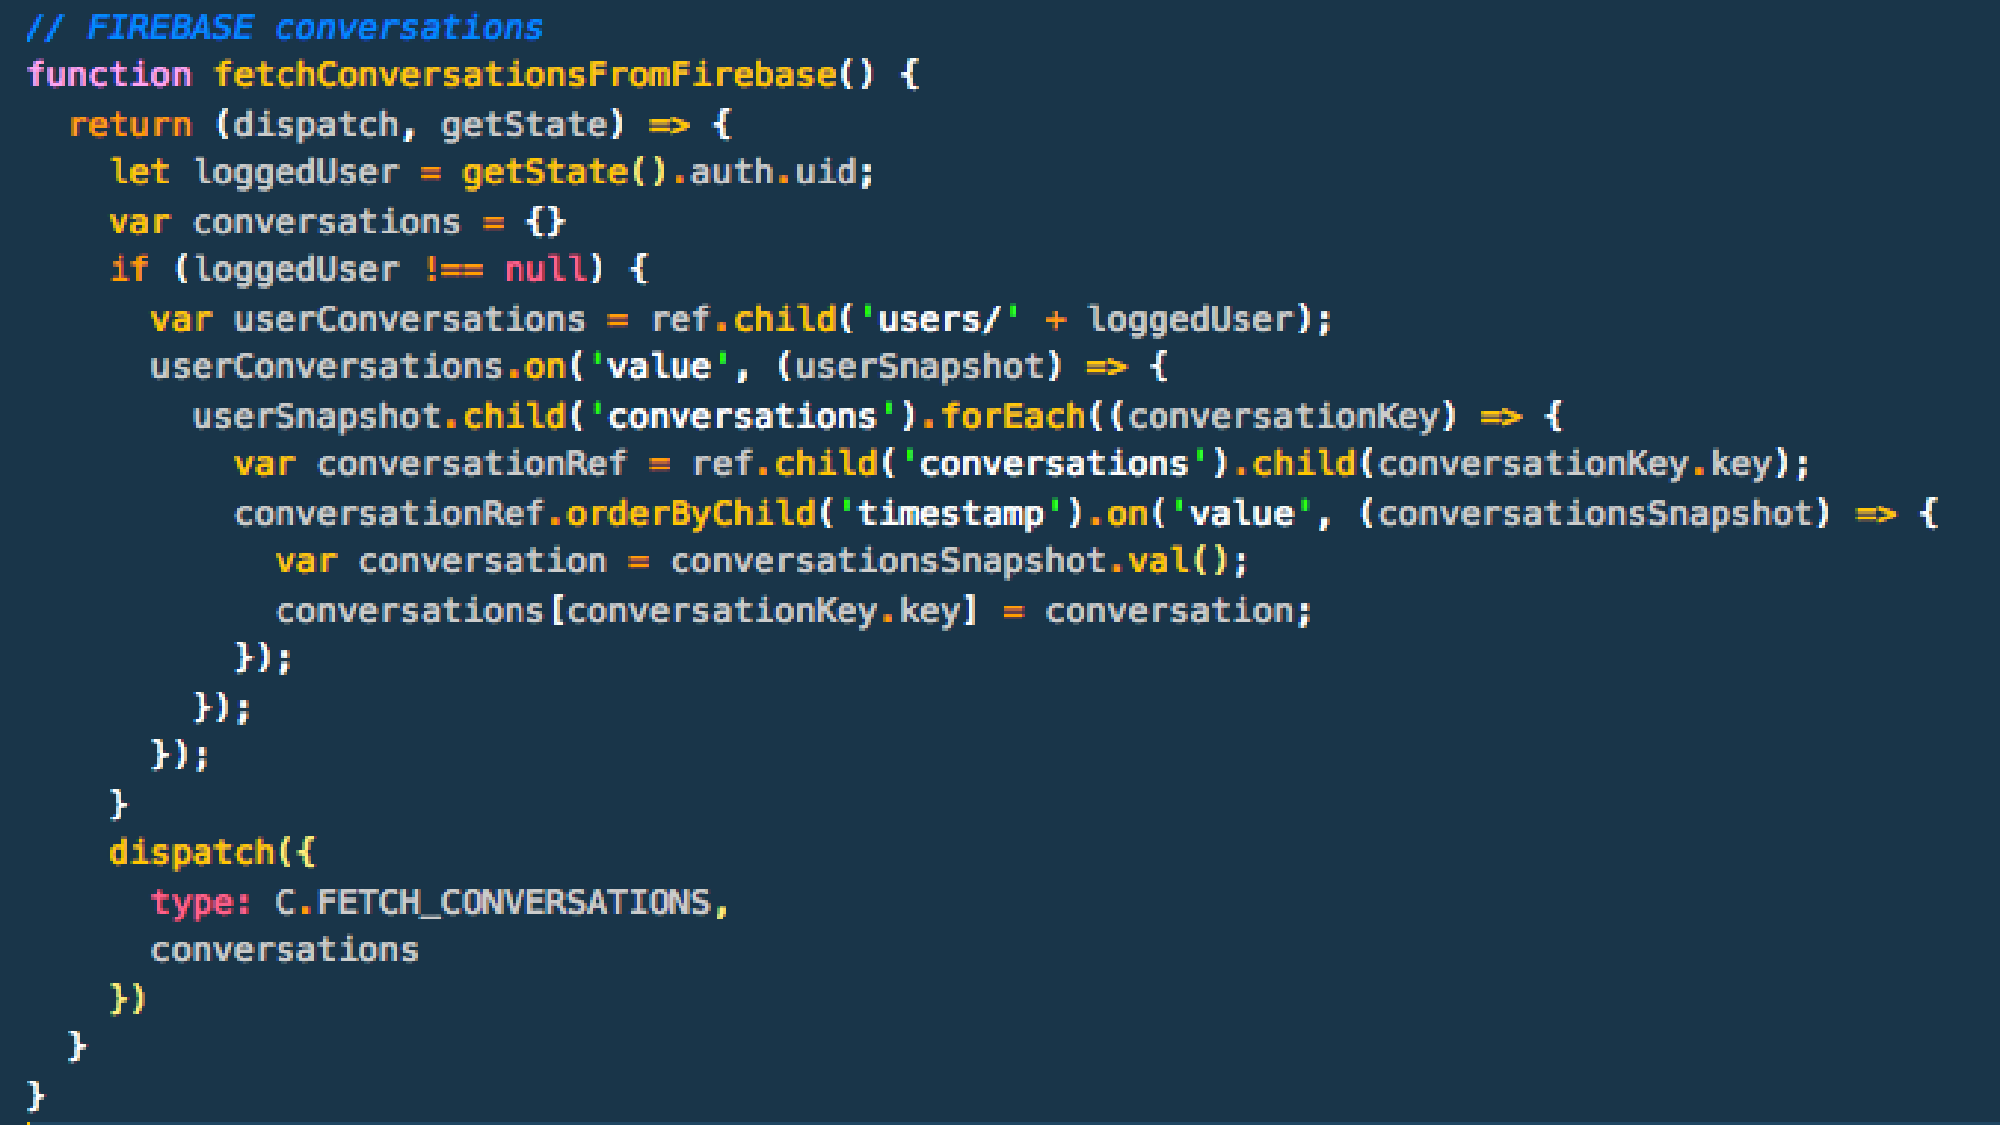
\includegraphics[width=1\textwidth]{figs/Fetch-conversation}
	\caption{Fetch conversation from Firebase}
	\label{fig:Fetch-conversation}
\end{figure}

This was difficult and we wasted a lot of time on learning how to do this. A lot of the Firebase documentation recommends doing a flat database structure precisely because of this, but we didn't quite get the concept of NoSQL databases until we stumble in a post  ~\cite{tutyuty}  which mentions denormalization, a concept that we completely understand the opposite way when learning about relational databases.

With Firebase a lot of the back-end code gets done on the client. To create a new user on Firebase, we needed to register in Firebase, after that, we needed to create the user inside the Users database and make sure to validate the information before adding it to the database. The back-end contains validation rules, however most of them are handled on the front-end. 

For the Participants JSON, we needed to get the Sender and the Receiver id. After that, we created a Conversation Key using Firebase Database Push method which gives the developer a unique key. After that, we added both users to the participant’s object as well as the conversation key to each of the Users object. This kind of seems repetitive but that’s one of the main reasons why Firebase is so fast. Because it only stores simple objects of string data.

The Messages functionality was the most intriguing and interest for us. We wanted to feel like a professional application, that's why we grabbed a lot of inspiration from the WhatsApp Web Client. We even created our bubbles inspired by theirs. Even though CSS is just a styling language it also gave us some lessons.  

It was a little bit complex to learn how to add new messages to the Conversation inside the Messages dictionary, again, it sounds counter intuitive but it did work as intended, we erased some of the sample information inside our Testing Firebase App, however we learn a lot in the process. Adding new messages was one of the most complex tasks, first we needed to get a new key from Firebase. Then if the conversation didn't exist we needed to create it. However, if it existed, we needed to get it from the Participants dictionary. The dictionary that contained both the sender and the receiver was the conversation that needed to get a new message. Again, this was another tricky part that we are proud of having solved.

Some remarks of our software development experience are also that the community in stack overflow and other IRC channels, were helpful. Also, there is a lot of people out there showing their contributions and doing open source code. That excites us a lot and makes us feel more challenged for the future.

Our conclusions for the implementation of the Web client are that we are very happy that we got the minimum functionality working, we wanted to do more as we showed on our initial timetable, however we now feel more experienced and we learned by firsthand the joy of developing with React. Which sounds like in the future is going to keep being useful (see React Virtual Reality ~\cite{4545etet}).


\subsection{Android Implementation}

As new programmers, we started by looking at existing Android messaging apps that use Firebase as a back-end so we could take ideas on how to start. There is a course in Udacity made by Google that makes a basic chat (all to all) that we used as reference for our app. ~\cite{4664rtyrtr67}.

Later on, we found out that this app was very different to what we needed. We needed a different database structure to be able to map each message to the appropriate conversation. With this came many complications. We had to change the whole structure of our program! We tried changing our code, but we found out that it was a hard task so we decided to start a new project from zero because it would be easier.
We had many problems during the way. One of our biggest challenge was to append a new message to the previous list of messages of a specific conversation.

The steps are:

\begin{itemize}
	\item Get the user id (the key) of the sender.
	\item Get the user id of the receiver.
	\item Search inside each “participants” children if the userid of the sender and receiver match the keys stored with a value of true.
	\item Get the “participants” children key that found before. This is the key for the conversation for the 2 participants.
	\item Go to ``messages" $\rightarrow$ ``key-found-in-previous-step" $\rightarrow$ append the message.
\end{itemize}

We focused on finishing the main activities of the chat and we were not able to implement a registration proccess.

We have different classes in our app:

\begin{itemize}
	\item \textbf{Chat}: Containing the instances of sender, receiver, senderUid, receiverUid, message and timestamp.
	
	\item \textbf{Chat-room}: This class is in charge of what happens inside the conversation. It already knows who the sender and receiver of the new message are and it finds out what were the previous messages of these 2 participants and appends the new message. 
	
	\item \textbf{LoginActivity}: This class is in charge of the log in process. In contrast with the other clients, a new user can only sign in and not sign up. The user can only sign in with an email and a password.
	
	\item \textbf{MainActivity}: This class is responsible for connecting everything in the app. It has many methods including a method that is responsible for getting and showing all the open conversations with the different users, a method that converts the receiver uId to the receiver name so it can display the name in screen.
	
	\item \textbf{User}: Class containing the instances of name, userId and email.
	
	\item \textbf{UserListActivity}: Class containing a method to get all the users from Firebase.

	\item \textbf{UsersArrayAdapter}: Special class made for android to be able to map a list of users to a list view. This was required because we needed to create a special model that contains the user class. We display the information via the cellprototype.xml that is attached to this class.
	
	\item \textbf{Participant}: 
	
	\item \textbf{ParticipantArrayAdapter}: 
	
\end{itemize}




\subsection{Testing}

For the testing process we were inspired by the verification and validation model (V- model), which is based on the relationship between each phase of the software development life cycle. Therefore, each development step is associate with a test phase.   The next figures summarise each phase of the methodology, which also is an integral part of our developed philosophy. 

\begin{figure}[ht]
\centering
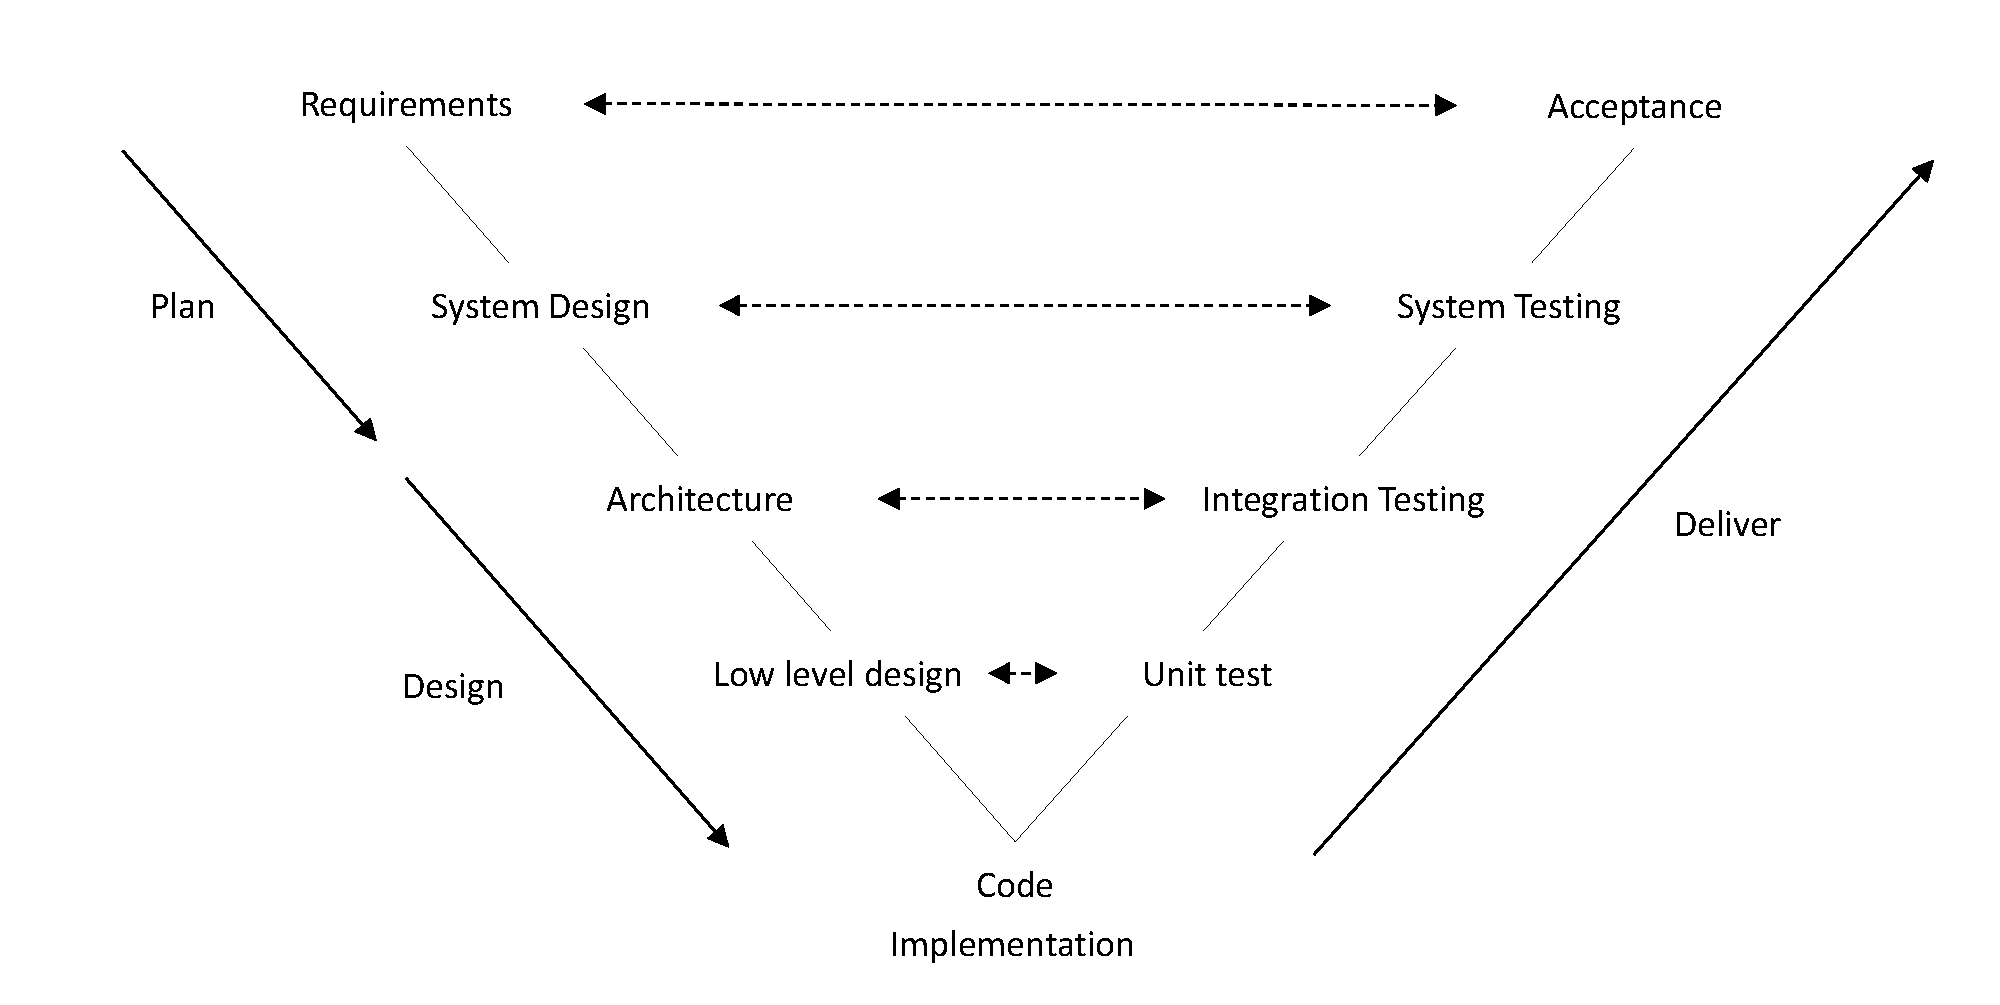
\includegraphics[width=1\textwidth]{figs/testing-met}
	\caption{Test foundation Methodology}
	\label{fig:testing}
\end{figure}


In spite of the fact that we were aware of the agile test methodology model (where each little division or task of software is tested while developing ~\cite{rtyeteey}), in our case we had to be flexible, considering our list of requirements by priorities. This means that the divisions of our software, as well as our architecture, change according to our learning curve across this project. Thus, our testing plan for each division of the software were extremely flexible from the beginning.

The next table presents the results of the testing process. An iterative process was conducted to guarantee a proper integration of the different clients.  Also, this process was challenging, considering that while we were trying to develop each client, at the same time we had to bear in mind the structure of the whole system.


\begin{table}[ht]
\caption{Requirements by priority level}
\label{tab:requirements}
    \begin{tabular}[c]{ | p{6cm} | p{3cm} | p{3cm} | p{3cm} |}
		\hline
		\centering\textbf{Feature} & \centering{\textbf{IOS}} & \centering\textbf{Web} & \centering\textbf{Android}  &
    \hline
    Log in & Ok & Ok & Ok \\
    \hline
    Log out & Ok & Ok & Ok \\
    \hline
    Registration & Ok & Ok &  No \\
    \hline
    Validate empty messages & Ok & Ok & Ok \\
    \hline
    Validate blank messages & Ok & Ok &  No \\
    \hline
    Render profile picture & Ok & Ok & No \\
    \hline
    Recover historical messages & Ok & Ok &  Ok \\
    \hline
    List of conversations & Ok & Ok &  Ok \\
    \hline
    Able to show long messages &  No & Ok & Ok \\
    \hline
    Conversation title & Ok & Ok & Ok \\
    \hline
    Contacts and message panel &  No & Ok &  No \\
    \hline
    Readable timestamp & Ok & Ok & Ok \\
    \hline
    HTTPS connections & Ok & Ok & Ok \\
    \hline
    Offline working & Ok & Ok & Ok \\
    \hline
    Get last message & No & Ok & No \\
    \hline
    Reset pasword & Ok & N.A. & No \\
    \hline
    \end{tabular}
\end{table}



From the above, we could state that our testing process was iterative across the development process as follows: 

\textbf{Initial Testing}.	Initial testing was the first test conducted on the application. The testing process began with the testing of the login unit/page that was demonstrated    during the initial presentation. At that point the testing was platform specific. There was no need for testing together across other platforms then. However, as the development progressed, our testing methodology was modified. 

\textbf{Development Phase Testing}.	These are the testing conducted through the development phase of the project.  The testing done during the development phase was such that the codes were shared amongst the team as soon as they were observed to be working and deleted or overwritten once it was found not to be working or not to meet our desired end. The testing was done intermittently as the project was being developed. The result of each test determined progression to the next phase. No member of the group was dedicated as a test engineer neither was any sub-team assigned the responsibility of testing the software. However, as each sub-team was working on its project, the test was also going on. Whoever was writing the code was a test engineer in his own right. Then when the team meets, the codes were run across platforms to query its compatibility and flexibility across platforms. The team members from the different platforms then criticise the codes based on their observations (\textbf{Red Teaming}) and suggested necessary modifications.

\textbf{Final/Integration Testing}. The final test was an integrated testing at the end of the project.  The final testing was done to ensure that all the users were able to carry out one to one conversation across the three clients’ platforms. At this stage, we encountered a challenge of the inability of the three clients’ bases to communicate directly with each other. However, the database structure was re-examined and the sub-teams developing the clients were made to restructure their back-end to follow the same format. Then, the inter-communications issue across the three platforms was resolved.   

\begin{figure}[ht]
\centering
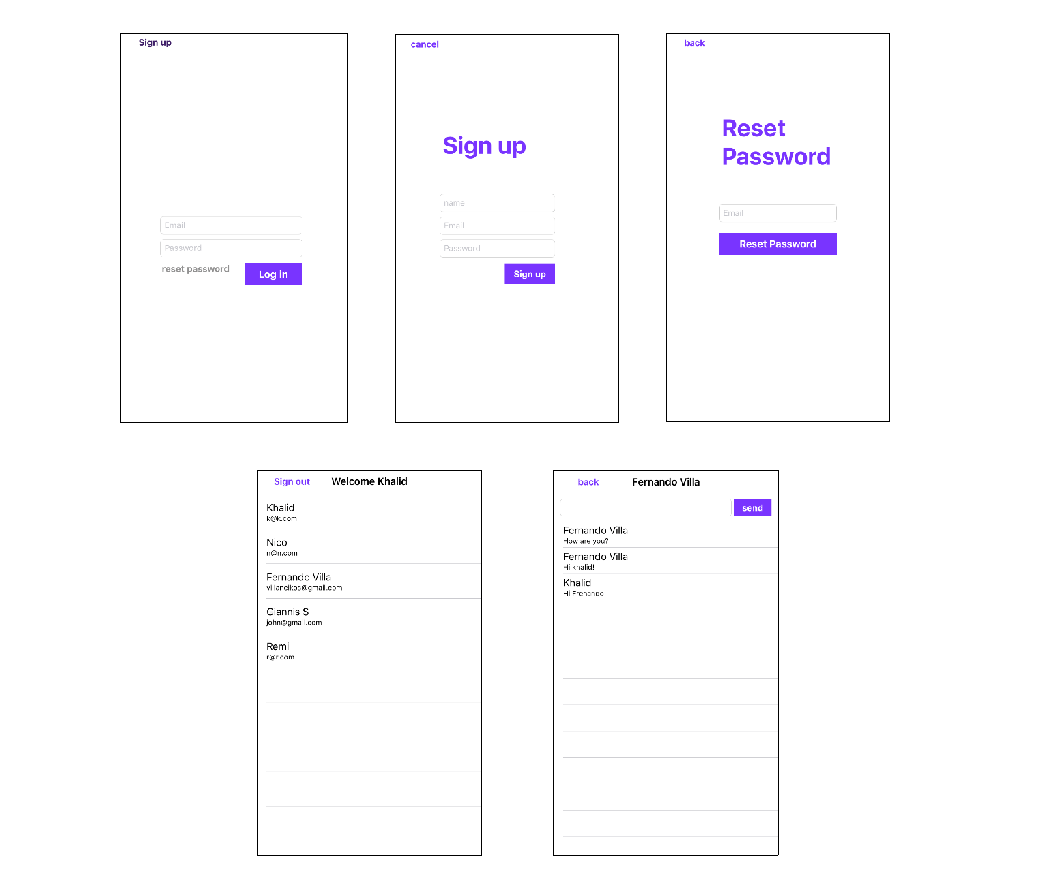
\includegraphics[width=1\textwidth]{figs/IOSscreen}
	\caption{iOS Screenshots }
	\label{fig:IOSscreen}
\end{figure}

\begin{figure}[ht]
\centering
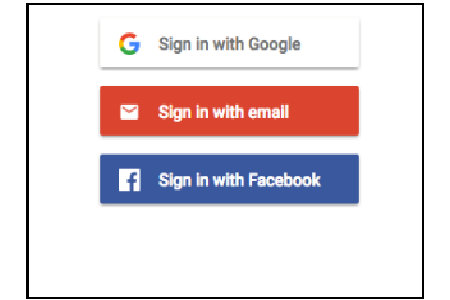
\includegraphics[width=0.3\textwidth]{figs/weblog}
	\caption{weblog }
	\label{fig:weblog}
\end{figure}

\begin{figure}[ht]
\centering
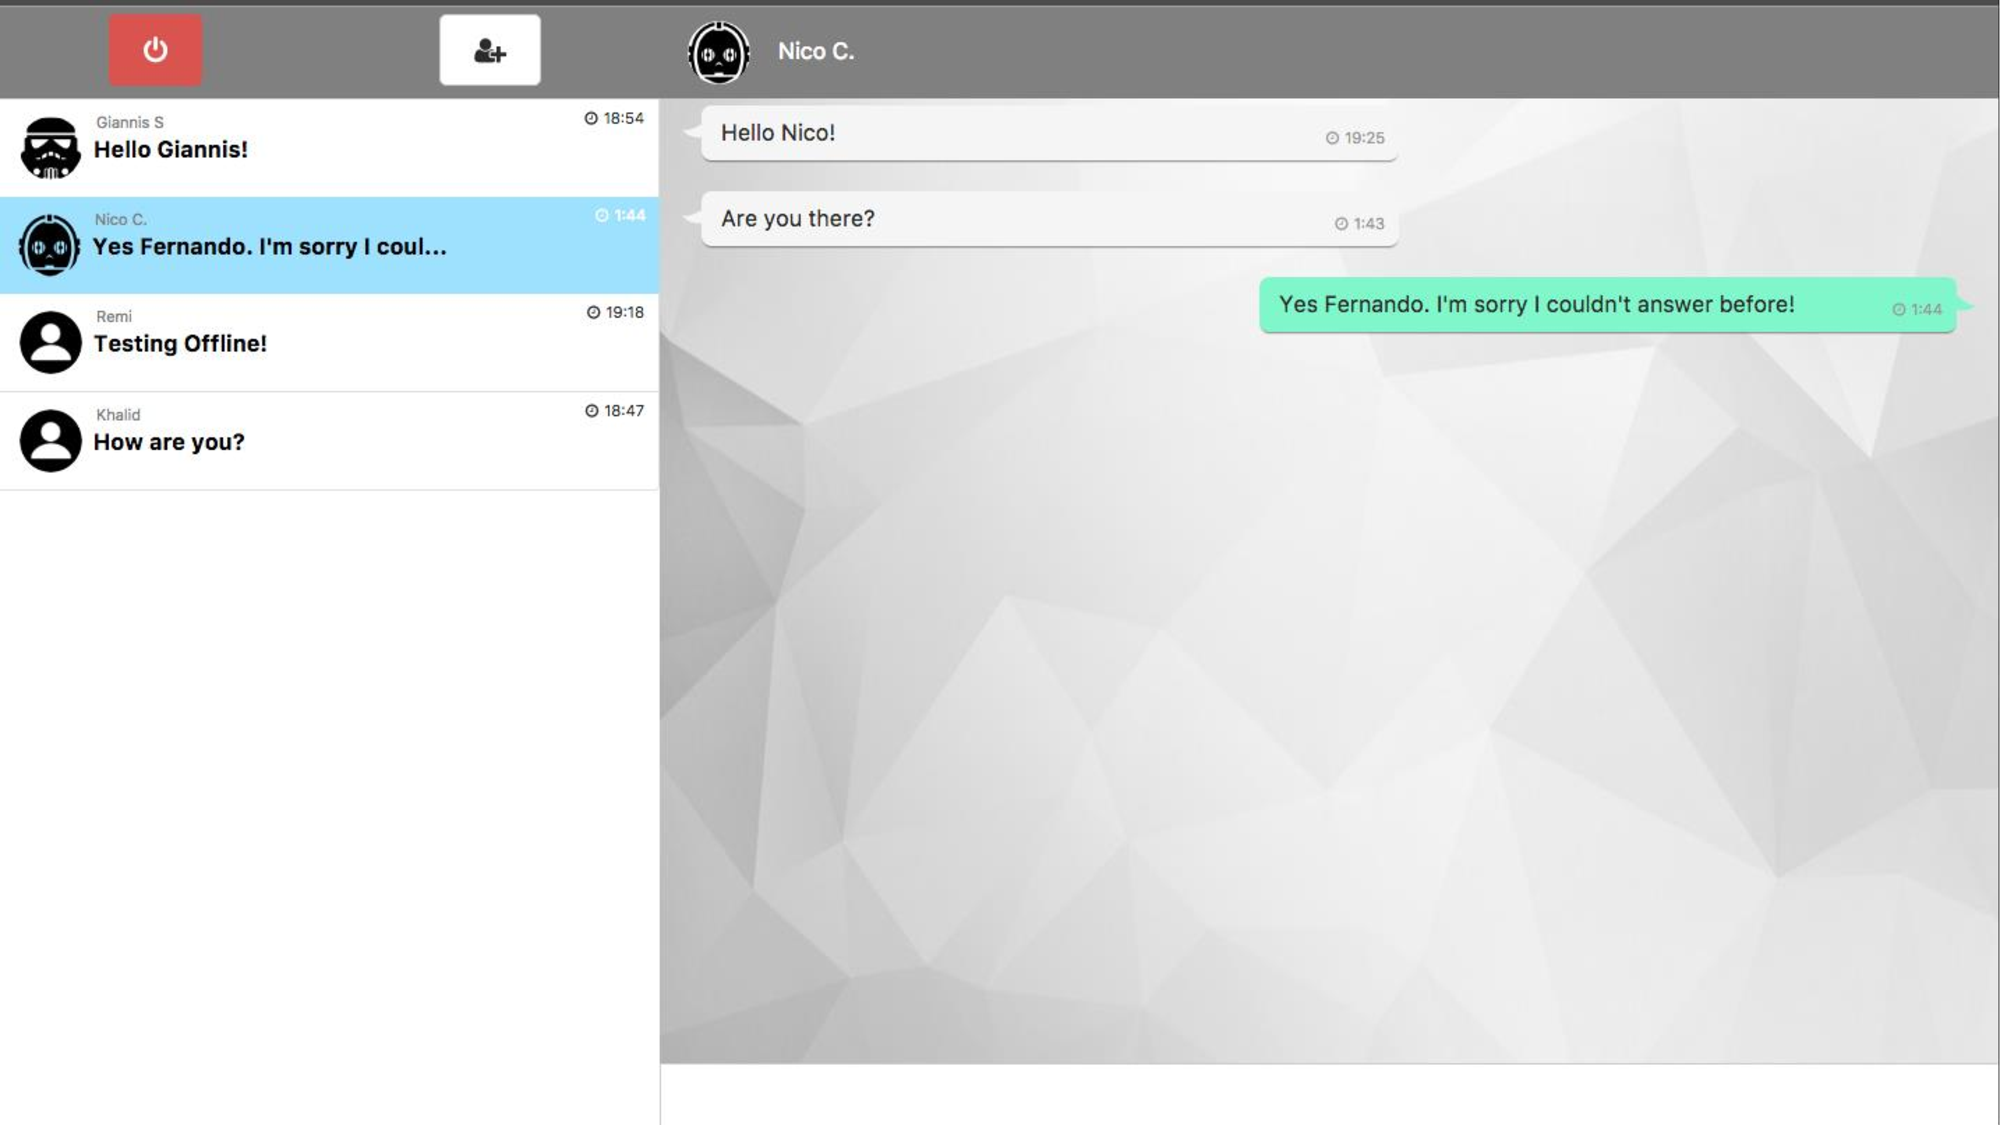
\includegraphics[width=1\textwidth]{figs/Chat-sample-Conversation}
	\caption{Chat-sample-Conversation }
	\label{fig:Chat-sample-Conversation}
\end{figure}

\begin{figure}[!t]
\centering
\subfigure[Main Screen]{
	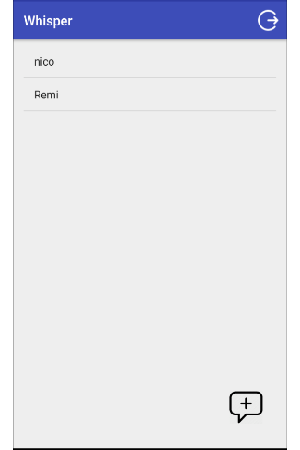
\includegraphics[width=0.3\textwidth]{figs/mainscreen}
	}
	\subfigure[Chat]{
	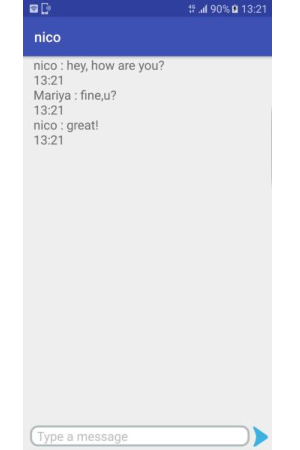
\includegraphics[width=0.3\textwidth]{figs/chatandroid}
	}
	\subfigure[Create New Conversation]{
	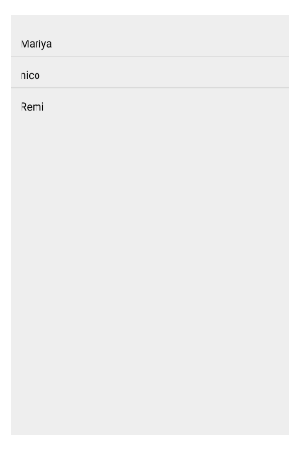
\includegraphics[width=0.3\textwidth]{figs/Newconversation}
	}
	\subfigure[Create New Conversation]{
	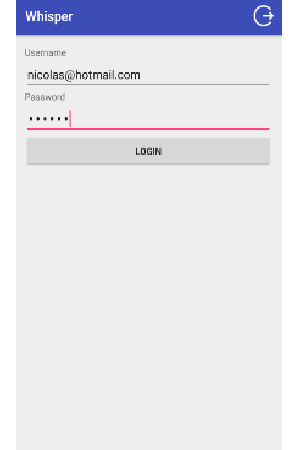
\includegraphics[width=0.3\textwidth]{figs/loginandroid}
	}
	\caption{Android Screenshots}
	\label{fig:android}
\end{figure}



\section{Team Work}
\label{sec:part 5}
The team worked together as described in the  two following sub-sections: i) Project organisation (structure of the team, where functionality and administrative task were assigned) and ii) Decision making and conflict resolution methodologies (i.e. How we make decisions and solve conflicts or disagreements as a team).

\subsection{Project Organisation}

5.1.1  Roles

All team members have two type of tasks: i) core tasks (e.g. programming goals) and ii) administrative tasks (e.g. documentation. In addition, the coordinator would be the officially communication channel of our team (i.e. our representative). However, it is clarified that this role does not imply a position of leadership or decision making (the decisions are made by the whole group following the decision making and conflict resolution methodology in section 2.4). The specific roles were already stated in the previous section (see Figure 2).

5.1.2.  Communication and work team tools.

\begin{itemize}
	\item Slack (for communication purposes and specific tasks).
	\item GitHub (for code sharing and version control).
	\item Compulsory weekly meeting every Monday (12:00 PM - 2:00 PM).
	\item Compulsory Google Hangout every Sunday (5:00 PM- 6:00 PM).
	\item Extra Google hangout meeting (when needed).
	\item Meeting on Wednesdays 2:00 PM- 5:00 PM (if needed). 
	\item A timetable and advance curve control (i.e. where we are vs where we ought to be).
	\item Our decision-making and conflict resolution methodology (Section 2.4).
	\item Learning meeting (each 15th day we discuss what we can improve as a team)
\end{itemize}


our activities are organised in the client development by hierarchy over the time. Thus, making the text message (which is mandatory) is more important than the image message (which is optional but highly desirable). Considering the above, we divide our horizontal tasks to develop each activity of the previous timetable, as follows.


\begin{figure}[ht]
\centering
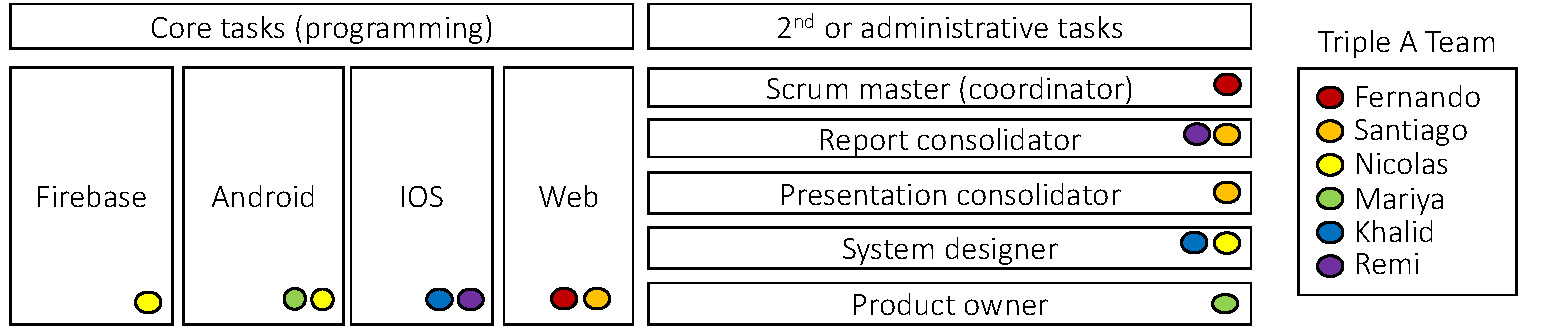
\includegraphics[width=1\textwidth]{figs/tasks}
	\caption{Tasks allocation}
	\label{fig:Tasks}
\end{figure}



5.2. Decision Making and Conflict Resolutions

Making agile agreements and rapidly solve conflicts is a key driver to maximise our team output. Our methodology is inspired in the agents and multiagent theory ~\cite{4646etyet}, specifically in a practical reasoning agent BDI (Belief – Desires - Intentions).

In this manner, each team member always have a valid point of view. Any difference between opinions is a deliberation process (where personal conflict is a conciliation process, which is a special type of deliberation), that would transform a set of options to a set of intentions (this implies that each time there is a deliberation process, the first step is to state a set of options). Then we will plan and assign resources. However, the deliberation process required a balance due to time restrictions (based on our timetable and curve advance). This implies that we must state a mechanism to accelerate the process wherever it is appropriated (deliberation process output is the ideal, but in a practical sense no always we will have time for a full consensus).

So, each time that we can't achieve a full consensus due to time restrictions, we have specified an agreement protocol that precipitated a final decision where the group will be move forward. For this, we use the \footnote{Borda Count: Each option receives $(m-1)$ points for each voter who vote as a first choice, $(m-2)$ for each voter who vote as a second choice, and so on, where $m$ is the number of options.  The winner option is that with more points. If there is a tie the decision will be random.} Borda Count vote procedure, to try to maximise the preferences of all the group.

Finally, for a personal conflict (such as a communication problem), there will be an arbitration protocol to try to solve it. Basically, the team identify those members that are no involving in the conflict in order that they can mediate. If after a conciliation process there is no any agreement, referees will make the decision (only if there are 2 or more referees). If referees declare itself unavailable to reach a final decision, then we will activate the agreement protocol. The following flowchart summarises our methodology.

\begin{figure}[ht]
\centering
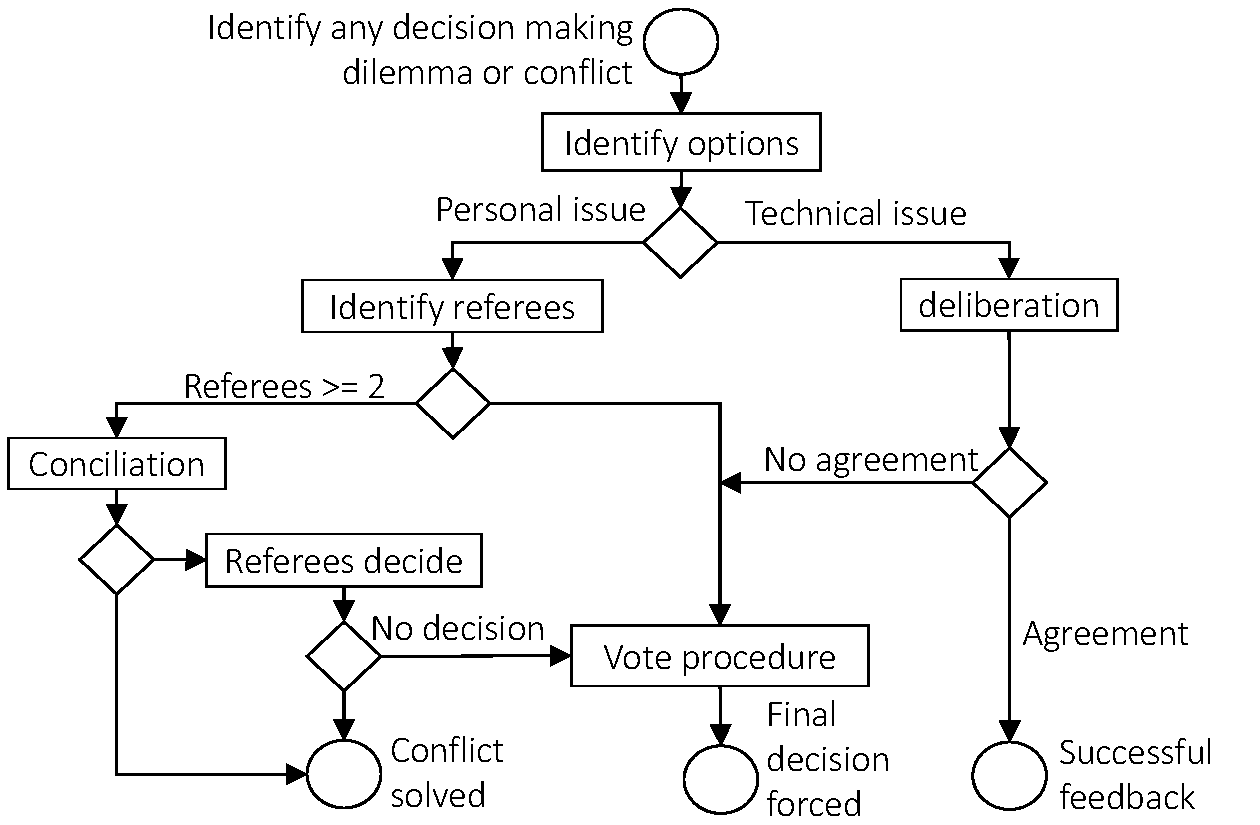
\includegraphics[width=0.6\textwidth]{figs/met}
	\caption{Decision Making and Conflicts Resolution Methodology}
	\label{fig:decisions}
\end{figure}




\subsection{Experiences while working together}

As earlier mentioned, we came from very different backgrounds and we are focusing on different career paths. It's a really good time to become more fluent in Software Engineering. Moreso, most of the industry is moving towards hiring more technically savvy people, that's why some of us picked this module even though it was not mandatory for us.

After learning what the project was going to be about, fortunately, we were interested in the same technologies such as Android and iOS so we split evenly on the different platforms that we were going to use. Each of us picked one technology that we were looking forward to learning in order to succeed in this project. However, that was also enough of a challenge but we succeeded.


For some of us, it was really stressful as we didn't even know how to use the terminal and even struggled with the GitHub command shell. Fortunately, we helped each other a lot and even got a small workshop in which we tested how to work with it.


We had our differences on some meetings. However, we always respected each others points of view and we worked out the overall best solution.
One of the most stressful moment was when we had to decide if we were in fact going to use Firebase. We had our doubts because we were unsure of the NoSQL database. But most of our doubts came from the lack of experience and because we didn't have a clear path towards the goal. We arrived at the conclusion that it is very stressful when you don't have adequate knowledge for the desired goal. 

In order to advance our knowledge as a fast as we could, we first started  reading about chat applications software on GitHub, Coursera, EdX, Udacity, and others.

For the iOS client development, we started with zero experience in Swift and Xcode. We started by building a simple portal to display grades and scores of students of an institution. It also has the feature of adding a new course and grade. With this simple project, we became more confident on developing iOS chat application, at least up to the level shown on this project. Our application was able to meet the requirements listed under our Priority 1 in Table 1 but for how to search for contacts and use Gmail. 
 
Agile Methodology requires dividing the project into small parts so that each part could be tested well before advancing. However, because we needed to learn and develop some skills while implementing, an ideal plan with proper small division was not achieved. 

Above all, we worked together well and we learnt a lot about current technologies and each other's background.



\section{Evaluation}
\label{sec:part 6}
What worked well: We've managed to have an accelerated learning curve that allowed us to meet the requirements and do a bit of extra work. Nevertheless, we have  to say that we wasted a lot of time trying to figure out a proper mechanism to work together and integrate all the parts in a single piece. In fact, as we have mentioned previously, work integration was our main challenge. 

Working as a team involved multiple challenges. Our different backgrounds and perspectives lead us to think on creative solutions. However, to develop properly that potential, a group project structure must be followed to succeed as a team. Some minor difficulties were agenda synchronisation and conciliating different point of views. 
During our execution, our plan changed a lot and we realised that planning in the initial stage of a project is essential for a good performance. In addition, we also learnt that to make a good plan that enable us to work as team, is not simple and requires experience and knowledge about software development. Its important to divide the tasks and properly allocate them. This could mean assigning each task to the person that knows most about it.

During the project we had to make many reevaluations of our plans. One good example of this is our decision of using Firebase and not create our back-end from scratch. After our first feedback, we had many evaluation to decided if it would be a good idea to continue using Firebase. This process induced more research and contrasting points of views, but finally we agreed to continue with our initial plan.

About our weakness and strengths as a team, this is a paradox in the sense that our principal strength is the diversity of professions, countries and languages, but this is also our weakness. Having different professional of multiple backgrounds, other than software engineering and computer science, gave to the group multiple perspectives and ideas. On the other hand, the deliberation process became more complex, and we lost in some situations “practical” reasoning as a group unit. In addition, these differences made the learning curve for this specific project much more challenging, but also way more rewarding at the end. 

As a group, we learnt a lot in the path and despite our knowledge disadvantage in developing, we managed to complete the main requirements for the distributed chat system. The application is far from complete in many senses. Some of the features we wanted to implement such as security and encryption can be improved, the android client doesn't work properly, different types of messages couldn't be added, such as images, videos, Gifts and documents. In addition, the structure of our database would make it easy to add the feature of a Group Chat. For a production-ready chat system, this project allows us to appreciate the complexity of this kind of system, as well as all the possibilities and features that can be added. Our chat, can be considered as an ``introduction" of a chat system and the opportunity areas that can be spotted. For instance, chat rooms, survey objects, user rating, etc. This without mention features like text recognition, an AI agent that helps you with daily tasks such as weather or exchange rates, or a proper design to recognise patterns of users that allow to improve continually the application (e.g. by using A/B testing, user habits and other browsing information).


\section{Peer assessment}
\label{sec:part 7}


\begin{table}[ht]
\caption{Requirements by priority level}
\label{tab:requirements}
    \begin{tabular}[c]{ | p{5cm} | p{5cm} | p{5cm} |}
		\hline
		\centering\textbf{Team Member} & \centering{\textbf{id}} & \centering\textbf{Mark} &
    \hline
    Fernando Villa & 1675380 & 17 \\
    \hline
    Nicolas Cabuli & 1651775 & 16.5 \\
    \hline
	Oluremi Obolo & 1141206 & 16.5\\
    \hline
    Nicolas Cabuli & 1651775 & 16.5 \\
    \hline
	Mariya Abdiyeva & 1673513 & 16.5 \\
    \hline
	Santiago Arrubla & 1666514 & 16.5 \\	
    \hline
	Khalid Alobaid & 1657587  & 17 \\
    \hline
    \end{tabular}
\end{table}


\bibliography{references}
\bibliographystyle{plain}
\end{document}
